\documentclass[12pt,letterpaper]{article}
%\topmargin 0in
%\textwidth 6in
%\textheight 9.0in
%\oddsidemargin 0.25in
%\evensidemargin 0.25in
% adjustment of page size
\addtolength{\textwidth}{30mm} %11pt: 20
\addtolength{\textheight}{30mm}
\addtolength{\voffset}{-15mm}
\addtolength{\oddsidemargin}{-15mm} %11pt: 7

\usepackage{epsfig}
%\usepackage{rotating}
\usepackage{subfigure}
\usepackage{amsmath}
\usepackage{amssymb}
\usepackage{dcolumn}
\usepackage{ccaption}
\usepackage{booktabs}
\usepackage{psfrag}
\usepackage{xspace}
\usepackage{html}
\usepackage{lineno}
\usepackage{setspace}
\usepackage{color}

%
% Macros for FCNC
%
%
% quark fields
\newcommand{\psibar}{\ensuremath{\overline{\psi}}\xspace}
\newcommand{\qbar}{\ensuremath{\overline{q}}\xspace}
\newcommand{\ubar}{\ensuremath{\overline{u}}\xspace}
\newcommand{\dbar}{\ensuremath{\overline{d}}\xspace}
\newcommand{\cbar}{\ensuremath{\overline{c}}\xspace}
\newcommand{\sbar}{\ensuremath{\overline{s}\xspace}}
\newcommand{\tbar}{\ensuremath{\overline{t}\xspace}}
\newcommand{\bbar}{\ensuremath{\overline{b}\xspace}}
\newcommand{\pbar}{\ensuremath{\overline{p}\xspace}}
\newcommand{\Wp}{\ensuremath{W^{+}}\xspace}
\newcommand{\Wm}{\ensuremath{W^{-}}\xspace}
\newcommand{\lh}{\ensuremath{{\mathrm{L}}}}
\newcommand{\rh}{\ensuremath{{\mathrm{R}}}}
\newcommand{\SUtwoL}{\ensuremath{\mathrm{SU(2)_{L}}}\xspace}
\newcommand{\UoneY}{\ensuremath{\mathrm{U(1)_{Y}}}\xspace}
\newcommand{\Uoneem}{\ensuremath{\mathrm{U(1)_{em}}}\xspace}
\newcommand{\VCKM}{\ensuremath{\mathbf{V}_\mathrm{CKM}}\xspace}
\newcommand{\Vud}{\ensuremath{V_\mathrm{ud}}\xspace}
\newcommand{\Vcd}{\ensuremath{V_\mathrm{cd}}\xspace}
\newcommand{\Vtd}{\ensuremath{V_\mathrm{td}}\xspace}
\newcommand{\Vus}{\ensuremath{V_\mathrm{us}}\xspace}
\newcommand{\Vcs}{\ensuremath{V_\mathrm{cs}}\xspace}
\newcommand{\Vts}{\ensuremath{V_\mathrm{ts}}\xspace}
\newcommand{\Vub}{\ensuremath{V_\mathrm{ub}}\xspace}
\newcommand{\Vcb}{\ensuremath{V_\mathrm{cb}}\xspace}
\newcommand{\Vtb}{\ensuremath{V_\mathrm{tb}}\xspace}

% Combinations of particles
\newcommand{\ccbar}{\ensuremath{{c\cbar}}\xspace}
\newcommand{\bbbar}{\ensuremath{{b\bbar}}\xspace}
\newcommand{\ttbar}{\ensuremath{{t\tbar}}\xspace}
\newcommand{\qqbar}{\ensuremath{{q\qbar}}\xspace}
\newcommand{\ppbar}{\ensuremath{{p\pbar}}\xspace}
\newcommand{\ee}{\ensuremath{{e^{+}e^{-}}}\xspace}
\newcommand{\mm}{\ensuremath{{\mu^{+}\mu^{-}}}\xspace}
\newcommand{\tautau}{\ensuremath{{\tau^{+}\tau^{-}}}\xspace}
\newcommand{\nunu}{\ensuremath{{\nu\overline{\nu}}}\xspace}
\newcommand{\ellell}{\ensuremath{{\ell^{+}\ell^{-}}}\xspace}
\newcommand{\Zee}{\ensuremath{{Z\rightarrow\ee}}\xspace}
\newcommand{\Zmm}{\ensuremath{{Z\rightarrow\mm}}\xspace}
\newcommand{\Zqq}{\ensuremath{{Z\rightarrow\qqbar}}\xspace}
\newcommand{\Wqq}{\ensuremath{{W\rightarrow q\overline{q}\,'}}\xspace}
\newcommand{\tZq}{\ensuremath{{t\rightarrow Zq}}\xspace}
\newcommand{\tZc}{\ensuremath{{t\rightarrow Zc}}\xspace}
\newcommand{\tZu}{\ensuremath{{t\rightarrow Zu}}\xspace}
\newcommand{\tWb}{\ensuremath{{t\rightarrow Wb}}\xspace}

% Math & symbols
\newcommand{\de}{\ensuremath{\mathrm{d}}}
\newcommand{\del}{\ensuremath{\partial}}
\newcommand{\delslash}{\ensuremath{\partial\!\!\!\!\!/}}
\newcommand{\Dslash}{\ensuremath{D\!\!\!\!\!/}}
\newcommand{\ra}{\ensuremath{\rightarrow}}
\newcommand{\LambdaQCD}{\ensuremath{\Lambda_{\mathrm{QCD}}}\xspace}
\newcommand{\alphas}{\ensuremath{\alpha_{S}}\xspace}
\newcommand{\costh}{\ensuremath{\cos\theta^*}\xspace}
\newcommand{\pt}{\ensuremath{p_{T}}\xspace}
\newcommand{\pT}{\pt}
\newcommand{\et}{\ensuremath{E_{T}}\xspace}
\newcommand{\Et}{\et}
\newcommand{\ET}{\et}
\newcommand{\mt}{\ensuremath{M_{T}}\xspace}
\newcommand{\Mt}{\mt}
\newcommand{\MT}{\mt}
\newcommand{\Ht}{\ensuremath{H_{T}}\xspace}
\newcommand{\HT}{\Ht}
\newcommand{\lshr}{\ensuremath{L_{\mathrm{shr}}}\xspace}
\newcommand{\xobs}{\ensuremath{\vec{n}_\text{obs}}\xspace}
\newcommand{\chisq}{\ensuremath{\textrm{top mass } \chi^2}\xspace}

% common units
\newcommand{\unit}[1]{\ensuremath{\:\mathrm{#1}}\xspace}
\newcommand{\statsyst}[2]{\ensuremath{\pm#1\mathrm{(stat.)}\pm#2\mathrm{(syst.)}\xspace}}
\newcommand{\stat}[1]{\ensuremath{\pm#1\mathrm{(stat.)}}\xspace}
\newcommand{\kev}{\unit{keV}\xspace}
\newcommand{\kevc}{\ensuremath{\unit{keV}/c}\xspace}
\newcommand{\kevcsq}{\ensuremath{\unit{keV}/c^{2}}\xspace}
\newcommand{\mev}{\unit{MeV}\xspace}
\newcommand{\mevc}{\ensuremath{\unit{MeV}/c}\xspace}
\newcommand{\mevcsq}{\ensuremath{\unit{MeV}/c^{2}}\xspace}
\newcommand{\gev}{\unit{GeV}\xspace}
\newcommand{\gevc}{\ensuremath{\unit{GeV}/c}\xspace}
\newcommand{\gevcsq}{\ensuremath{\unit{GeV}/c^{2}}\xspace}
\newcommand{\tev}{\unit{TeV}\xspace}
\newcommand{\invfb}{\unit{fb^{-1}}}
\newcommand{\invpb}{\unit{pb^{-1}}}


% Names
\newcommand{\sm}{standard model\xspace}
\newcommand{\eps}{\ensuremath{\varepsilon}\xspace}
\newcommand{\lumi}{\ensuremath{\mathcal{L}}\xspace}
\newcommand{\br}{\ensuremath{\mathcal{B}}\xspace}
\newcommand{\xsect}{cross section\xspace}
\newcommand{\xsects}{cross sections\xspace}
\newcommand{\ie}{i.e.\ }
\newcommand{\eg}{e.g.\ }
\newcommand{\Zj}{$Z$+jets\xspace}
\newcommand{\Zbb}{$Z\bbbar$+jets\xspace}
\newcommand{\Zcc}{$Z\ccbar$+jets\xspace}
\newcommand{\Znj}{$Z$+$n$\,jets\xspace}
\newcommand{\Wj}{$W$+jets\xspace}
\newcommand{\Wnj}{$W$+$n$\,jets\xspace}
\newcommand{\btag}{$b$-tag\xspace}
\newcommand{\pyth}{{\sc Pythia}\xspace}
\newcommand{\VminusA}{\ensuremath{V\!-\!A}\xspace}
\newcommand{\alp}{ALPGEN\xspace}
\newcommand{\Lint}{\ensuremath{\int\!\mathcal{L}\de t}\xspace}

% For Algebra
\def\bz{\ensuremath{{\mathcal B}_Z}}
\def\bw{\ensuremath{{\mathcal B}_W}}
\def\lum{\ensuremath{\!\int\! {\mathcal L}dt}}
\def\tt{\ensuremath{\sigma_{t \bar{t}}}}
\def\alj#1{\ensuremath{{{\mathcal A}_{LJ}}_\textrm{#1}}}
\def\rlj#1{\ensuremath{{\mathcal R}_\textrm{#1/ww}}}
\def\betaz{\ensuremath{{\mathcal B}_\textrm{z}}}

%%% Local Variables: 
%%% mode: latex
%%% TeX-master: t
%%% End: 

\sloppy
% Comment the next two lines for official drafts.
\pagewiselinenumbers
\doublespacing

\captionnamefont{\small\bfseries}
\captiontitlefont{\small\mdseries}
\captiondelim{:\,\,}%{\hskip 2ex}}
\hangcaption

\newcommand{\clearemptydoublepage}{\newpage{\pagestyle{empty}\cleardoublepage}}

\begin{document}

\thispagestyle{empty}
\vspace*{-0.5in}
\begin{flushright}

CDF/PHYS/TOP/CDFR/$8833$ \\
\today\\
\end{flushright}
\vspace{0.5in}
\begin{center}
\begin{huge}
{\bf Search for the Flavor Changing\\[1mm] Neutral Current Decay \boldmath\tZq\unboldmath}
\end{huge}
\end{center}
% Authors and institutions
\vspace{0.5in}
\begin{center}
\begin{large}

{Charles Plager, David Saltzberg, Michael Sutherland}\\
{\em University of California, Los Angeles}\\[5mm]

{Melissa Franklin, Ingyin Zaw}\\
{\em Harvard University}\\[5mm]

{Jennifer Lindsay Gimmell}\\
{\em University of Rochester}\\[5mm]

{Ulrich Husemann, Paul Tipton}\\
{\em Yale University}\\[5mm]

\end{large}
\end{center}

%\renewcommand{\baselinestretch}{1}
\normalsize

% Abstract
\vspace{5mm}

% Jennifer's recent change: abstract text moved to abstract.tex
\begin{abstract}
  We search for the flavor changing neutral current decay of the top
  quark \tZq with $1.12\invfb$ of data. This decay is extremely rare in 
  the \sm, and a signal at the Tevatron would be an indication 
  of new physics. Using $Z+\ge4$ jet candidate events with and without a loose
  secondary vertex \btag, we expect an upper limit on the branching 
  fraction of $7.1\pm3.0\%$.

\end{abstract}

%  We search for the flavor changing neutral current decay of the top
  quark \tZq with $1.12\invfb$ of data. This decay is extremely rare in 
  the \sm, and a signal at the Tevatron would be an indication 
  of new physics. Using $Z+\ge4$ jet candidate events with and without a loose
  secondary vertex \btag, we expect an upper limit on the branching 
  fraction of $7.1\pm3.0\%$.


\clearemptydoublepage

\tableofcontents

\clearemptydoublepage

% Introduction
\section{Introduction}
In the \sm of particle physics (SM), flavor changing
neutral current (FCNC) decays are highly suppressed. They
do not occur at tree level, and are only 
allowed at the level of quantum loop corrections at very 
small branching fractions, as shown in CDF Note 7744~\cite{CDF7744}. 
The branching fraction for the top quark decay \tZq is predicted 
to be $\mathcal{O}(10^{-14})$, far below the experimental sensitivity 
of the Tevatron or even the Large Hadron Collider (LHC). As summarized 
by J.A.\ Aguilar-Saavedra~\cite{Aguilar-Saavedra:2004wm}, there exist 
new physics models that predict much higher branching fractions, 
up to $\mathcal{O}(10^{-2})$. Any detection of top's FCNC decay at the 
Tevatron would be an indication of new physics. 

We search for \ttbar events in which either top quark decays via 
the FCNC to a $Z$ boson and a quark ($u$ or $c$), and
the other top quark decays via the SM to a $W$ boson and a $b$ quark.  We
examine the decay channel in which the $Z$ subsequently decays to a
pair of charged leptons (\ee or \mm), and the $W$ decays to two
quarks. We also evaluate the case in which both tops decay via FCNC, and
take into account its impact on the signal acceptance. Although the branching 
fraction of $Z\rightarrow\ee/\mm$ is only 3.33\% per channel, 
it is a very clean channel to identify that there was a $Z$ present in the 
decay. We chose the \Wqq decay mode because it has the highest branching 
ratio and contributes to a final state with a large jet multiplicity.  
Thus, the final signature is a reconstructed $Z$ and four or more jets, 
one of which is a $b$-jet that can be identified using a loose secondary vertex 
(SECVTX) \btag. Our experimental signature does not include any neutrinos in the
final state, and we are therefore able to fully reconstruct the event.

The dominant background contribution for this analysis comes from
$Z$s produced in association with jets (\Zj). The other 
background contribution comes from SM $\ttbar\to\Wp b\, \Wm \bbar$
events. In the dilepton decay mode, the invariant mass of two leptons
forms a continuum background to the $Z$ peak, and in the lepton+jets
decay mode, the invariant mass of the lepton and a jet that is
misidentified as a lepton may fall within the Z mass window.  There is
a contribution similar in size from electroweak production of pairs of
gauge bosons, or ``dibosons'', where we consider both $WZ$ and $ZZ$ events. 
The contribution from $W$s produced in association with jets (\Wj) and
the $WW$ diboson production is negligible.


% Description of analysis method
\section{Method}
We perform a blind search for the FCNC decay \tZq, with the signal
region defined as events with a reconstructed $Z$ in the mass range of
76--106\gevcsq, four or more jets, and mass \chisq (constructed from
reconstructed $W$, SM top, and FCNC top masses) less than 9. We split
the data sample into two subsamples that are analyzed separately, a
loose SECVTX $b$-tagged and an anti-$b$-tagged sample. We take the signal
acceptances and efficiencies from a Monte Carlo (MC) simulation with
appropriate scale factors and trigger efficiencies applied. We then 
normalize the expected number of signal events to the lepton+jets
top cross section. The dominant background for the signal
region comes from \sm \Zj production, in which we estimate using a rigorous 
combination of data and Monte Carlo techniques. Other background contributions 
include SM top and dibosons, estimated using MC simulation, and \Wj production,
estimated using both data and MC simulation.

The event selection for the $b$-tagged and the anti-$b$-tagged data samples
are optimized for the best combined expected limit. We use both
Feldman-Cousins (FC) and Bayesian frameworks for calculating expected
limits. Both frameworks take systematic uncertainties into account 
in the limit calculation. We find that the limits obtained in either 
framework track each other well. As the limit calculation in the FC 
framework is very CPU-intensive, we optimize our selection criteria 
for the best expected limit using the Bayesian framework and use the 
FC framework to obtain the limit for our signal event yields.  After
the final selection criteria have been chosen, we derive a limit on
the branching fraction of the decay \tZq from the number of events
observed in the signal region and the number of expected background
events.


% Data Sample and Event Selection
\section{Data Sample and Base Event Selection}
For this analysis, we use data collected with the CDF II detector
between March 2002 and September 2006, which corresponds to an
integrated luminosity of $1.12\invfb$. We exclude runs 179057--186598
(``compromised COT'' period) and runs prior to 150145 for muons in the
CMX detector (no triggering on CMX possible).  The data we analyzed
for this analysis was collected with inclusive lepton triggers that
require $\et > 18\gev$ for electrons (datasets \texttt{bhel0d},
\texttt{bhel0h}, and \texttt{bhel0i}) and $\pt > 18\gevc$ for muons
(datasets \texttt{bhmu0d}, \texttt{bhmu0h}, and \texttt{bhmu0i}). We
apply CDF's Good Run List version~16~\cite{GoodRun16},
and require that the data from the silicon detector, electromagnetic
calorimetry, and muon chambers to be marked ``good''. In addition to
data marked good from the muon chambers, we also remove the runs in
which the CMX detector is ignored.
%We also remove the runs without the CMX detector ourselves.

We begin by selecting events with two leptons which form a $Z$, and
four or more jets. We then separate the sample into events with a
loose SECVTX \btag and anti-tagged events. We then further optimize the
selection criteria to obtain the best expected limit and place further
requirements upon the jets \et, transverse mass \mt, and a mass
$\chi^2$.

\subsection{Selection Criteria}
For the base event selection we require exactly one lepton pair of the
same flavor and opposite charge. For \Zee, one of the leptons is a tight 
central electron and the other is a tight central electron, a tight phoenix
electron, or a tight track lepton.  For \Zmm, one of the leptons is a
tight central muon, and the other is a tight central muon or a track
lepton.  The difference in the $z$-coordinate of the point of closest
approach to the beam line, $\Delta z_0$, of the two legs is required to be
less than $5\unit{cm}$, and the dilepton invariant mass is required
to be between 76\gevcsq and 106\gevcsq.

\subsection{Lepton Selection}
This analysis will use tight central electrons, tight
phoenix electrons, and tight central (CMUP or CMX) muons which follow the 
standard CDF Joint Physics criteria for electrons~\cite{JPElectron} and 
muons~\cite{JPMuon}. The selection criteria are listed in 
Tables~\ref{table:TCE}, \ref{table:PHX}, and \ref{table:muons}.
For the selection of tight track leptons, we use the requirements determined for
the lepton+track top \xsect measurement~\cite{CDF8696}, as shown in
Table~\ref{table:tracks}. In addition, we impose a correction for 
electron+track $Z$ candidates to account for possible energy loss due to 
bremsstrahlung. In this case, a collinear photon will deposit energy into a 
nearby calorimetry tower. We can use the energy from the photon to recover 
the energy loss of the track. For these tracks, we use \et if it is larger than \pt.


\subsection{Jet Selection}
In addition to the $Z$ candidate, we require 4 or more jets with
$\et> 15\gev$ corrected to jet energy correction level 5 and $|\eta|
\leq 2.4$. In events with five or more jets, only the four leading
jets are considered. Events with $Z+\geq 4$ jets fall into our signal region and
are therefore blinded. We use the events with a $Z$ and three or fewer
jets as our control region to perform cross-checks for our background
prediction methods. For some studies, we will shrink the blind signal
region by applying a cut on a mass $\chi^2$ variable.
 
\subsection{Additional Selection Criteria}
After the base selection, we apply further cuts to improve the
background rejection. These cuts are optimized for the best expected
limit. We found that a ``sliding'' cut on the transverse energy of the
four leading jets, a cut on the transverse mass of the system, \mt, and a
mass $\chi^2$ are the most sensitive. The definitions of these variables, 
calculation of the expected limit, and the subsequent optimization of 
the additional selection criteria are described in 
Section~\ref{section:limitsandoptimization}.

\subsubsection{``Sliding'' Jet Transverse Energy}
The FCNC signal comes from the decay of massive top quarks and
contains four hard jets. Therefore a ``sliding'' cut on the transverse
energies of the four leading jets in an event suppresses background
from \Zj events that originates from a lower energy process and from
SM \ttbar, where two of the four jets have to come from initial or
final state radiation. 
%We found a cut of $\et>40\gev$ for the leading
%jet, $\et>30\gev$ for the second leading jet, $\et>20\gev$ for the
%third leading jet, and $\et>15\gev$ for the fourth leading jet to be
%optimal for both the anti-$b$-tagged and the $b$-tagged analysis.

\subsubsection{Transverse Mass}
A second variable with good discriminating power is the
transverse mass of the full event, defined as
\begin{equation}
  \mt = \sqrt{ \left(\sum\et \right)^2 - \left(\sum\vec{p}_{T}\right)^2 },
\end{equation}
where the sums include the four leading jets and the reconstructed $Z$. 

\subsubsection[Mass $\chi^2$]{Mass \boldmath $\chi^2$\unboldmath}
\label{section:masschi2}
We make use of the ability to fully reconstruct the event kinematics to
separate signal from background by constructing a mass $\chi^2$
variable. In a signal event, there is one decay of the type \tWb.
Two jets in the event form a $W$, which in turn form a top quark together with
a third jet. There is also one decay of the type \tZq, in which the
$Z$ has to be paired with the fourth jet to form the second top. The mass
$\chi^2$ is defined as

\begin{equation}
\chi^2 = 
\left(\frac{m_{W,\mathrm{rec}} - m_{W,\mathrm{PDG}}}{\sigma_{W, rec}} \right)^2 +
\left(\frac{m_{\tWb,\mathrm{rec}} - m_{t,\mathrm{PDG}}}{\sigma_{\tWb}} \right)^2 +
\left(\frac{m_{\tZq,\mathrm{rec}} - m_{t,\mathrm{PDG}}}{\sigma_{\tZq}} \right)^2,
\end{equation}

where, for each permutation, the masses are obtained by the following prescription:

\begin{enumerate}
\item Correct the four leading jets four-vectors with level-5 jet energy scale
  corrections and top-specific corrections taken from the Top Mass
  Template (TMT) analysis~\cite{CDF7532}.
\item Calculate the invariant mass of the first two jets to form the mass
  of the reconstructed $W$, $m_{W,\mathrm{rec}}$.
\item Vary the momentum four-vectors of both $W$ daughters within their respective
  resolutions such that the $W$ mass is fixed to its PDG value. The
  resolutions are taken from the TMT analysis.
\item Calculate the invariant mass of the $W$ and the third jet to form the reconstructed
  top mass, $m_{\tWb,\mathrm{rec}}$.
\item Reconstruct a $Z$ from two leptons.
\item Fix the $Z$ mass to its PDG value by varying the two lepton four-vectors. We 
  assume the lepton's resolutions are a constant percentage of their total momenta.
\item Calculate the invariant mass of the $Z$ and the fourth jet, 
  $m_{\tZq,\mathrm{rec}}$.
\end{enumerate}

In the above calculation for the mass $\chi^{2}$ distribution, we assume a top mass
of 175\gevcsq. The widths shown are the RMS values of the HEPG-matched reconstructed
signal Monte Carlo, where $\sigma_{W, rec}$, $\sigma_{\tWb}$, and $\sigma_{\tZq}$
are 15\unit{GeV}, 24\unit{GeV}, and 21\unit{GeV}, respectively. The above prescription 
is repeated for all possible permutations of the four leading jets in the event, and 
the permutation with the lowest $\chi^2$ is selected. We do not make use of $b$-tagging 
information in resolving the combinatorics.

%: $\sqrt{\chi^2} < 1.35$ for anti-tagged
%events, and $\sqrt{\chi^2} < 1.6$ for loose SECVTX tagged events. 

\subsubsection{Lepton+Jets Selection}
Our expected number of signal events are normalized to the lepton+jets SECVTX
\xsect. The lepton+jets analysis searches in \ttbar pairs for the standard model 
top decay \tWb, where one top decays hadronically and the other leptonically 
yielding the lepton + three or more jets + missing \Et event signature. They require one 
tight lepton (TCE, CMUP, CMX), three jets with $\Et>20\gev$ corrected to jet 
energy correction level 5, and at least two loose SECVTX $b$-tags. Details of their acceptance 
selection criteria are given in Table~\ref{table:LepJets}.

%After optimizing our event selection for the best expected limit, we
%make further requirements for our events. We require higher transverse
%energy for the highest four jets to be greater than 50\gev, 40\gev,
%30\gev, and 20\gev, respectively. We also require the scalar sum of
%the \et s (\pt s) of the leptons and the \et s of the jets to be above
%260\gev. We also require the mass $\chi^2$, which measures the
%deviations of the masses of the reconstructed FCNC top, W, and SM top
%from the average in matched Monte Carlo events, to be less than
%5x.x.



% Signal Monte Carlo
\section{Signal Expectation}
Our signal expectation is quantified through both an acceptance, composed
of a geometric acceptance and a pre-tagged efficiency, and an 
efficiency of the \btag for the $b$-tagged sample. The following
section describes the signal MC generation with helicity re-weighting,
and the calculations of acceptance and efficiency for the signal.

\subsection{Event Generation}
We have generated the FCNC signal MC samples using the \pyth event
generator, version 6.216~\cite{Sjostrand:2003wg}, for the $1.12\invfb$
run range (runs 141544--222426) and a top mass of $175\gevcsq$. The
FCNC decay \tZq is not in the list of standard decays within
\pyth; therefore, we have redefined the decay products of the $t
\rightarrow W d$ decay channel, which has a negligible branching fraction, 
to be a $Z$ boson and a $c$ or $u$ quark. 

For the main FCNC signal sample, we force one top quark into the SM
decay \tWb and the other top quark to our FCNC decay \tZc
letting \pyth decide randomly whether the
$t$ or $\tbar$ decays to a $W$ and a $b$ quark.  This decay is the
dominant contribution to the FCNC signal acceptance.  We have
generated 0.1 events per $0.5\unit{nb^{-1}}$, yielding a total of
539,445 signal events. The decay of the $Z$ is forced into \ee or
\mm pairs, and the decay of the $W$ is forced into \Wqq.

In addition to the main FCNC signal MC sample, we generated samples 
to study special cases for events with an FCNC decay. We generated a sample
to study the additional acceptance gained from events where both top quarks 
decay via the FCNC decay, or the ``double FCNC decay''. In the double FCNC sample, 
we do not force either of the $Z$ decays; therefore, each $Z$ can decay into \ee, 
\mm, and $q\qbar$ independently of the other. We generated a restricted-decay sample
where the $Z$ and the $W$ forced to decay leptonically, and another sample where we 
allow the fully inclusive decays of the $Z$ and the $W$.


We also generated a sample where the $c$ quark is replaced by a $u$ quark to 
study the small reduction of the $b$-tagging efficiency. Each sample was generated 
with 0.1 events per $1\unit{nb^{-1}}$, for a total of approximately 110,000 events 
per sample, and spans the full run range. All signal MC samples are listed in more detail in 
Table~\ref{table:MCsamples}.

\begin{table}[t]
\begin{center}
\caption{\label{table:MCsamples} List of Monte Carlo samples generated.
The abbreviation ``incl'' refers to the inclusive decay of the boson shown.}
\vspace{2mm}
\small\begin{tabular}{l l  D{,}{,}{-1} l} 
\toprule
{\bf \ttbar Decays}
& {\bf Sample Name}
& \multicolumn{1}{c}{\bf Sample Size}
& {\bf Description } \\ 
\midrule
$ZcWb$ & $Z(ll)W(q\overline{q}')$    & 539,445 & Signal Monte Carlo Sample: \Zee  \\
       &                             &         & or \Zmm, and \Wqq\\

$ZcWb$ & $Z(ll)W(l\nu)$              & 111,181 & \Zee or \Zmm  \\
       &                             &         & and $W\rightarrow e\nu$, $W\rightarrow \mu\nu$, 
                                                  or $W\rightarrow \tau\nu$ \\ 

$ZcWb$ & $Z(incl.)W(incl.)$          & 116,573 & Inclusive $Z$ and $W$ decays\\


$ZcZc$ & $Z(ll,\qqbar)Z(ll,\qqbar)$  & 116,573 & Double FCNC decay: \Zee, \Zmm \\
       &                             &         & or $Z\rightarrow \qqbar$ \\


$ZuWb$ & $Z(ll)uW(q\overline{q}')$   & 116,573 & \Zee or \Zmm \\
       &                             &         & and \Wqq \\

\bottomrule
\end{tabular}
\end{center}
\end{table}


%We have also generated smaller test samples with 50,000 events each in
%order to study two special cases, the case when both top quarks decay
%via the FCNC decay, and the case of an FCNC decay into a $Z$ and a $u$
%quark.  We use these samples to study the
%additional acceptance gained from the double FCNC decay and the small
%reduction in the $b$-tagging efficiency when the $c$ quark is replaced
%by a $u$ quark. In the double FCNC sample, the two $Z$ bosons are
%independent and cannot be forced into correlated decay
%mode. Therefore, each $Z$ can decay into \ee, \mm, and $q\qbar$
%independently of the other.

%We have also generated two test samples with 100,000 events, covering the full 
%run range, for the FCNC decay, one with no restrictions on the decay channel for 
%the W and Z bosons and the other with $Z$ decaying to \ee or \mm, and $W$ 
%decaying to a lepton and its corresponding neutrino.

%The decay to a $c$ is expected to be dominant. In addition, we are
%not specifically tagging the $c$ quark so the analysis remains
%general. The only effect is that the presence of the $c$ quark makes
%the efficiency to tag the events slightly higher even though the
%tagging efficiency is dominated by the presence of the $b$ quark from
%the SM decay.

\subsubsection{Helicity of the Decay Vertex}
Due to the fact that we have redefined the $t \rightarrow W d$ decay
channel and redefined the decay products of the FCNC decay, \pyth
does not know the type of interaction involved at the decay
vertex. Hence \pyth decays the particles isotropically in their rest
frame, \ie flat in \costh, the cosine of the angle between the top
boost direction and the isospin $-1/2$ lepton.  Fig.~\ref{fig:costheta}a 
shows the \costh distribution of the FCNC top decays in the FCNC signal MC.
Note that the distribution for \costh is not flat, but linear in $\theta^*$.
We correct for this by fitting a straight line to the distribution, and 
using the difference from the linear fit we assign a weight. More details 
on this procedure are seen in section~\ref{section:helicitysystematics}.

\begin{figure}[t]
  \begin{center}
  \subfigure[]{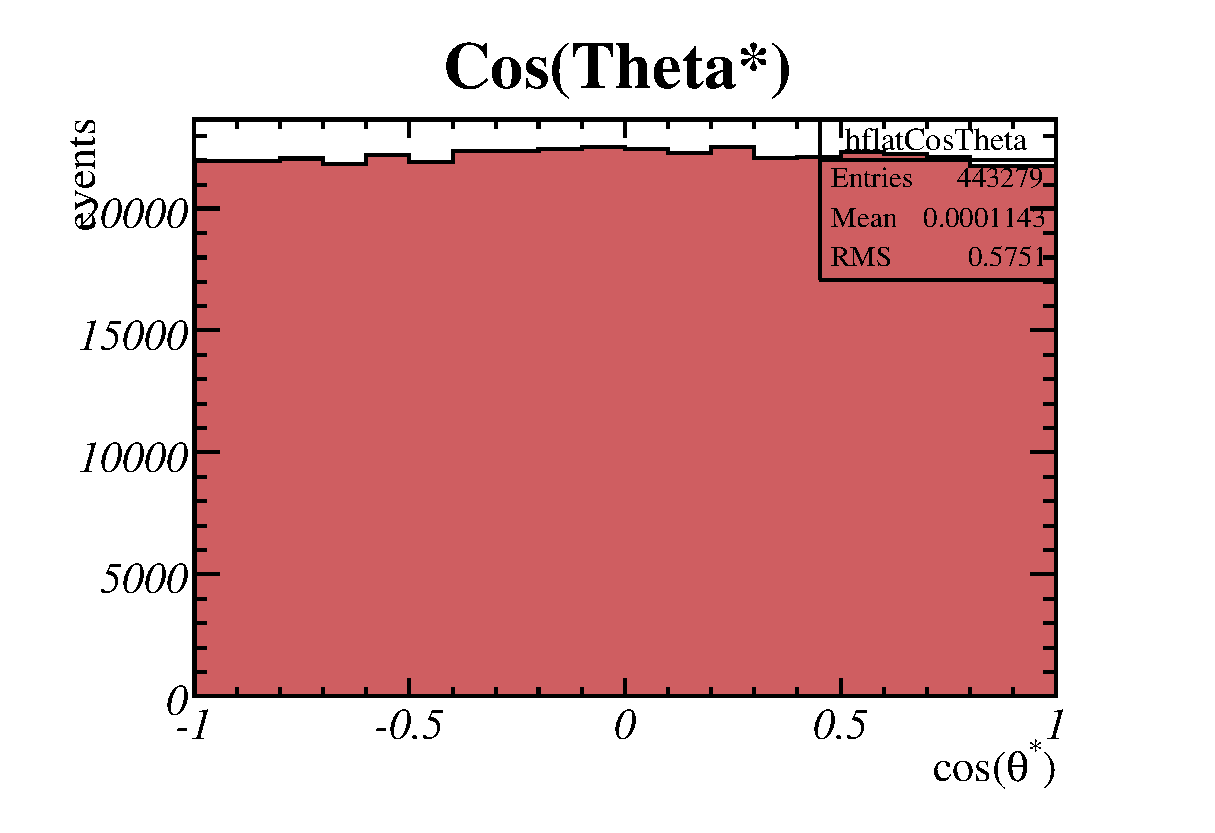
\includegraphics[width=0.48\textwidth]{pics/CosThetaA.eps}}
  \subfigure[]{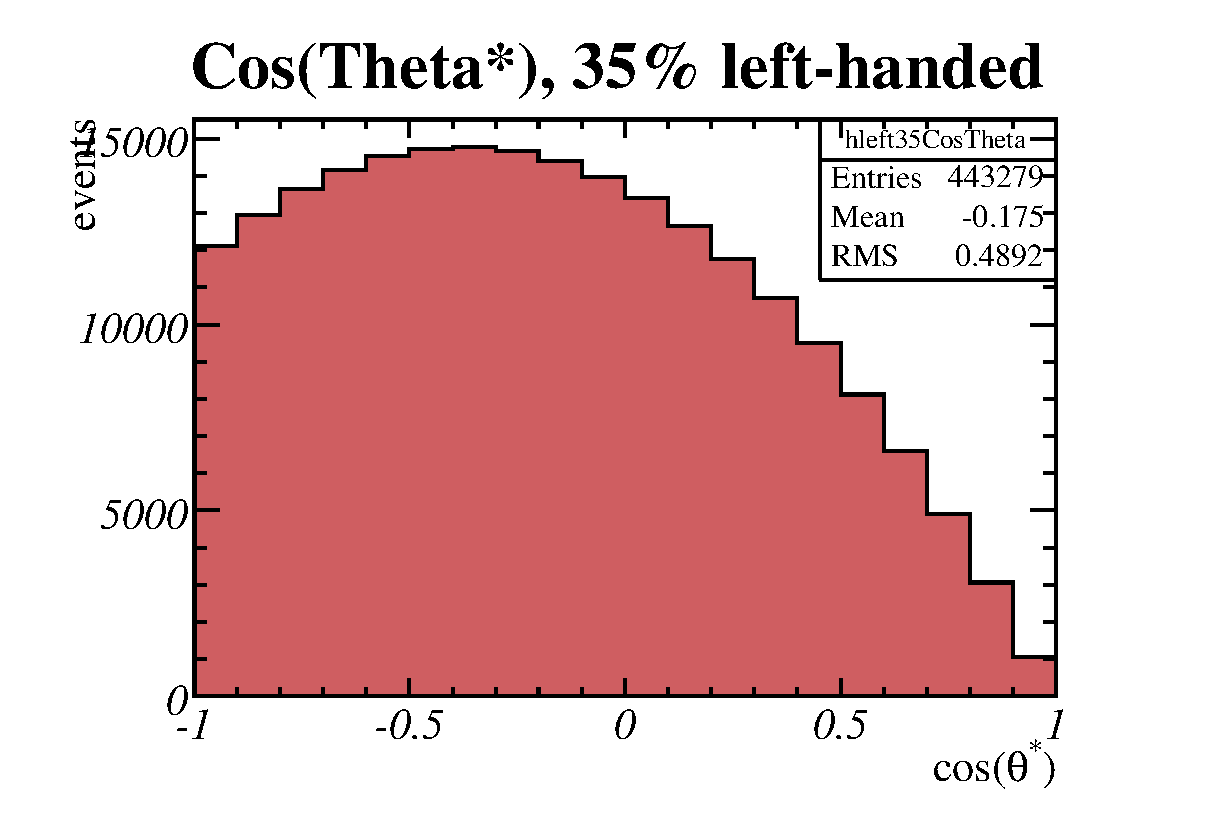
\includegraphics[width=0.48\textwidth]{pics/CosThetaB35left.eps}}
\end{center}
  \caption{Distribution of \costh for the
    FCNC signal MC sample: (a) before re-weighting, (b) after re-weighting
    according to a $Z$ helicity of 65\% longitudinal and 35\%
    left-handed.}
  \label{fig:costheta}
\end{figure}

The helicity of the $W$ from a SM top decay is determined by the fact
that the longitudinal degree of freedom of the $W$ is acquired from the
Higgs field. Any theory beyond the SM must provide a similar mechanism
to create massive gauge bosons; therefore, the best guess for the longitudinal
fraction of the $Z$ helicity, $f^0$, is given by the SM prediction~\cite{Tait}:

\begin{equation}
f^0 = \frac{m_t^{~2}}{2m_Z^{~2} + m_t^{~2}} \approx 0.65.
\end{equation}

The Higgs mechanism does not predict the fraction of left-handed to
right-handed helicity; however, for a $Z$ decay, changing from
left-handed to right-handed is equivalent to looking at the oppositely
charged lepton.  Assuming that the CDF detector is approximately
symmetric with respect to positively and negatively charged leptons,
the acceptance is very similar when switching from a
left-handed to a right-handed decay.

For all acceptance calculations, we re-weight the signal MC sample such
that the $Z$ helicity is 65\% longitudinal and 35\% left/right-handed. Our
ignorance of the exact nature of the interaction is taken into account
by a assigning a corresponding systematic uncertainty, as will be
described in Section~\ref{section:helicitysystematics}.


\subsection{Acceptance}

\subsubsection{Acceptance and Scale Factors}
The acceptance for the FCNC signal MC is determined by applying the
baseline event selection ($Z$ candidate and four jets with $\et>15
\gev$ and $|\eta| <$ 2.4) to the signal MC and then correcting for some known limitations of
the MC simulation. 
%The raw acceptance for our decay channel is 16.79 $\pm$ 0.05\% (stat). 
%When the branching fractions for $Z \rightarrow$ \ee, \mm and \Wqq are taken 
%into account, we get a raw acceptance of 0.76$\pm$0.004\%.

For the $Z$ reconstruction efficiency we have to
take into account the discrepancy between the efficiency to identify a
lepton in data and the MC simulation. These scale factors are not only different for the
different detectors used to identify the leptons, but they also vary among the MC
simulations corresponding to different data taking periods. We apply these scale 
factors on a per-event basis, and take into account the added efficiency from
recovering tight leptons as tracks. Each event receives a scale factor, ${\mathcal SF}$:

\begin{eqnarray*}
{\mathcal SF} & = & \mathcal{SF}_{L1} \cdot \mathcal{SF}_{L2} 
               +  (1-\mathcal{SF}_{L1}) \cdot \mathcal{SF}_{L2} \cdot \mathcal{SF}_{T1} 
               +  (1-\mathcal{SF}_{L2}) \cdot \mathcal{SF}_{L1} \cdot \mathcal{SF}_{T2}. \\
\end{eqnarray*}

In the above equation, ${\mathcal SF}_{L1}$ and ${\mathcal SF}_{L2}$ are the scale factors
for the leptons, and ${\mathcal SF}_{T1}$ and ${\mathcal SF}_{T2}$ are the track scale factors
for the tracks matched these leptons. The added efficiency from recovering both tight 
leptons as tracks appears in the last two terms of the above equation. Note that for 
the case where neither lepton has been matched to a track, both $\mathcal{SF}_{T1}$ 
and $\mathcal{SF}_{T2}$ are zero, and the above equation reduces to the more familiar 
event scale factor for a $Z$ formed from two tight leptons:

\begin{eqnarray*}
{\mathcal SF} & = & \mathcal{SF}_{L1} \cdot \mathcal{SF}_{L2}. \\
\end{eqnarray*}

It is possible to apply the same treatment for the lepton and track trigger efficiencies. 
We ignore the trigger efficiency gain from recovering tight leptons as tracks. Instead, we
assume that all tight leptons fire the trigger, and that phoenix electrons and tracks
would not have. Per event, we assign a weight for the trigger efficiency, 
${\mathcal E}$:

\begin{eqnarray*}
{\mathcal E} & = & \mathcal{E}_{L1} + \mathcal{E}_{L2} 
                        -  \mathcal{E}_{L1} \cdot \mathcal{E}_{L2}. \\
\end{eqnarray*}

In the above efficiency equation, ${\mathcal E}_{L1}$ and ${\mathcal E}_{L2}$ are the trigger 
efficiencies for leptons. The lepton ID scale factors and lepton 
trigger efficiencies are given in Table~\ref{table:sf}. The corrected acceptances for our 
signal Monte Carlo samples are given in Table~\ref{table:acc_cor}.

%Since these scale factors are
%different for the different detectors we use to identify leptons, we
%divide our $Z$ sample by the lepton type of the two legs, CEM, PHX,
%CMUP, CMX (arches or miniskirt/keystone), and track lepton. Then we apply the relevant 
%scale factors to each category. In addition, we apply correction factors for the 
%lepton trigger efficiencies for each lepton type. We only allow tight central electrons and 
%tight muons to trigger. 

%The scale factors for the different detectors are
%given in Table~\ref{table:sf}. In addition there are slight
%differences between the trigger simulation in the MC and the data,
%taken into account via the trigger efficiencies for tight central
%electrons and muons, see Table~\ref{table:e_eff} and
%Table~\ref{table:mu_eff}.
%The raw and
%corrected $Z$ reconstruction efficiencies for the different $Z$ types
%is given in Table~\ref{table:raweff}. 
%Our overall acceptance for the base selection criteria is
%$\mathcal{A}(\ttbar\to Zc\,Wb) = ??$.

\begin{table}[t]
\begin{center}
\caption{\label{table:acc_cor} The corrected acceptances for the FCNC signal Monte Carlo samples in \%,
  shown with statistical uncertainties only.}
\vspace{2mm}
\small\begin{tabular}{c D{;}{\pm}{-1} D{;}{\pm}{-1} D{;}{\pm}{-1} D{;}{\pm}{-1}} 
\toprule
\multicolumn{1}{c}{\bf MC Sample Name }
& \multicolumn{1}{c}{\bf Acceptance } 
& \multicolumn{1}{c}{\bf BR(Z) } 
& \multicolumn{1}{c}{\bf BR(W/Z) } 
& \multicolumn{1}{c}{\bf Acc$\times$BR}\\ 
\midrule
$Z(ll)W(q\overline{q}')$   & 15.95;0.05 & 6.73;0.01 & 67.60;0.27 & 0.73;0.00 \\
$Z(ll)W(l\nu)$             & 2.50;0.05  & 6.73;0.01 & 32.40;0.27 & 0.05;0.00 \\
$Z(ll,\qqbar)Z(ll,\qqbar)$ & 14.76;0.45 & 6.73;0.01 & 69.91;0.06 & 1.39;0.04  \\
\bottomrule
\end{tabular}
\end{center}
\end{table}

\subsubsection{Branching Fractions}
In the FCNC signal MC simulation, we generate \ttbar 
events with one top decaying via the FCNC mode and the other via the \sm 
mode. Ultimately, we are interested in setting a limit on ${\mathcal B}(\tZq)$. 
We have to properly translate the acceptances for \ttbar $\rightarrow 
Zc Wb$ and \ttbar $\rightarrow Zc Zc$ to extract the limit for \tZq. In order to do this, 
we assume ${\mathcal B}(t \rightarrow Wb) + {\mathcal B}(t \rightarrow Zc) = 1$. The different 
decay modes for the \ttbar pair are as follows:
%\begin{center}

\begin{displaymath}
\begin{array}{|r|cc|}
\hline
                                & {\mathcal B}(t \rightarrow Wb) &
{\mathcal B}(t \rightarrow Zc) \\
\hline
{\mathcal B}(t \rightarrow Wb) & {\color[rgb]{0, 0.5, 0}\bw \cdot \bw} &
{\color[rgb]{0, 0, 0.5}\bw \cdot \bz} \\
{\mathcal B}(t \rightarrow Zc) & {\color[rgb]{0, 0, 0.5}\bw \cdot \bz} &
{\color[rgb]{0.5, 0, 0}\bz \cdot \bz} \\
\hline
\end{array}
\end{displaymath}
%\\ \vspace*{-.1in}

where

%\\ \vspace*{-.3in}
\begin{eqnarray*}
\bz & \equiv & {\mathcal B}(t \rightarrow Zc) \textrm{,} \\
\bw & \equiv & {\mathcal B}(t \rightarrow Wb) = 1 - \bz  \textrm{, and} \\
{\color[rgb]{0, 0.5, 0}\bw \cdot \bw} & \textrm{is} & \textrm{the SM \ttbar background.}
\end{eqnarray*}
%\\ \vspace*{-.0in}
%\end{center}

From this, we can derive the number of events we expect, namely,

%\begin{center}
%\vspace*{-.25in}
\begin{eqnarray*}
{\mathcal N}_\textrm{signal} &=& \left( {\color[rgb]{0, 0, 0.5}2 \bz (1
- \bz)} \cdot {\mathcal A}_{WZ} + {\color[rgb]{0.5, 0, 0}\bz^2} \cdot
{\mathcal A}_{ZZ} \right) \cdot \sigma_{t \bar{t}} \cdot \int {\mathcal
L} dt\\
&=& \bz
           \underbrace{ \left( {\color[rgb]{0, 0, 0.5}2 (1 - \bz)} +
{\color[rgb]{0.5, 0, 0}K_{ZZ/WZ} \cdot \bz} \right)}_\textrm{Acceptance
Correction Factor} \cdot
           \overbrace{{\mathcal A}_{WZ}}^\textrm{From MC}  \cdot
\sigma_{t \bar{t}} \cdot \int {\mathcal L} dt,\\
\end{eqnarray*}
%\\ \vspace*{-.1in}

where

%\\ \vspace*{-.3in}
\begin{eqnarray*}
{\mathcal A}_{WZ} & \equiv & \textrm{Acceptance } \cdot \textrm{
efficiency for } t \bar{t} \rightarrow WbZc \textrm{, and} \\
{\mathcal A}_{ZZ} & \equiv & \textrm{Acceptance } \cdot \textrm{
efficiency for } t \bar{t} \rightarrow ZcZc \textrm{, and} \\
K_{ZZ/WZ} & \equiv & \textrm {Ratio of } {\mathcal A}_{ZZ} \textrm{ to }
{\mathcal A}_{WZ} \sim 2 \textrm{ (from MC)}.\\
\end{eqnarray*}

%\end{center}
As shown in the following algebraic expressions, we normalize
to the measured lepton+jets top cross section. Note that the lepton+jets
SECVTX cross section top cross section measurement assumes that the 
top quark can only decay as expected by the SM, \tWb. Consequently, 
we have adjust the lepton+jets top cross section for acceptance 
changes due to possible FCNC top decays. In the algebra that follows, we
show that including the FCNC decay mode to the lepton+jets top
cross section yields an acceptance correction expression that 
is based on the limit we set for the FCNC decay. 
We say that this acceptance correction ``runs'' with the \tZq limit.

We also account for the FCNC signal falling within the SM top cross section
acceptance. We use the top cross section event selection to measure the 
acceptance both in a special FCNC signal MC sample with inclusive decays of 
the $W$ and $Z$, $Z(incl.)W(incl.)$, and in the double FCNC MC sample,
$Z(ll,\qqbar)Z(ll,\qqbar)$.


%Like the previous measurement, we are normalizing to the measured
%lepton+jets SECVTX top cross section. The top cross section
%measurement assumes that the top quark decays only to
%$Wb$. 

%Consequently, we have adjust the top cross section based on the
%limit we set for the FCNC decay. We also account for the FCNC signal
%falling within the top cross section acceptance by measuring the
%acceptance with the top cross section event selection on the Monte
%Carlo sample where one top decays to $Zc$ and the other to $Wb$, where
%we allow all decays of the $Z$ and $W$ bosons and the Monte Carlo
%sample where both tops decay to $Zc$.
  
The formula for the top cross section measurement is given by

\begin{displaymath}
{\tt}_\textrm{``Lepton + Jets''} =
  \frac {{\mathcal N}_{LJ} - B_{LJ}}{{\mathcal A}_{LJ} \cdot \lum},
\end{displaymath}
where \alj{~} is acceptance convoluted with efficiency.
We modify the acceptance to allow for the FCNC decay.

\begin{eqnarray*}
\alj{~}&=& (1-\betaz)^2\cdot\alj{ww} + 2\cdot\betaz(1-\betaz)\cdot\alj{wz}
+ \betaz^2\cdot\alj{zz}\\
&=& \alj{ww} \cdot \left[(1-\betaz)^2 + 2\cdot\betaz(1-\betaz)\cdot\rlj{wz}
+ \betaz^2\cdot\rlj{zz}\right]\\
\end{eqnarray*}
%\\ \vspace*{-.25in}

where

%\\ \vspace*{-.2in}
\begin{eqnarray*}
\rlj{wz}&\equiv&\frac{\alj{wz}}{\alj{ww}}\\
\rlj{zz}&\equiv&\frac{\alj{zz}}{\alj{ww}}\\
\end{eqnarray*}
%\\ \vspace*{-.3in}
This gives an enhancement to the top cross section as shown below.

\begin{eqnarray*}
{\tt}_\textrm{``Lepton + Jets''}
  & = &   \frac {{\mathcal N}_{LJ} - B_{LJ}}
{{\mathcal A}_{LJ} \cdot \lum} \\
  & = & \overbrace{\frac{1}
{(1-\betaz)^2 + 2\cdot\betaz(1-\betaz)\cdot\rlj{wz} + \betaz^2 \cdot
\rlj{zz}}}^
\textrm{Enhancement Factor}\\
& &{\bf \cdot} \underbrace{\frac {{\mathcal N}_{LJ} - B_{LJ}}
{\alj{ww} \cdot \lum}}_\textrm{Standard Cross Section} \\
\end{eqnarray*}
Inserting this top cross section back into our calculation for the
number of events gives

\label{eq:fullacc}
\begin{eqnarray*}
{\mathcal N}_\textrm{signal} &=& \bz
           \left( 2 (1 - \bz) + K_{ZZ/WZ} \cdot \bz \right) \cdot
           {\mathcal A}_{WZ} \cdot \\
& & \sigma_{t \bar{t}} \cdot \int {\mathcal L} dt\\
&=&  \bz
           \left( 2 (1 - \bz) + K_{ZZ/WZ} \cdot \bz \right) \cdot
           {\mathcal A}_{WZ} \cdot \\
& & 
  \frac{1}
{(1-\betaz)^2 + 2\cdot\betaz(1-\betaz)\cdot\rlj{wz} + \betaz^2 \cdot
\rlj{zz}}
{\bf \cdot} \frac {{\mathcal N}_{LJ} - B_{LJ}}
{\alj{ww} \cdot {\color[rgb]{0, 0.5, 0} \lum}} \cdot {\color[rgb]{0,
0.5, 0}\lum} \\
&=&  \bz {\bf \cdot}
  ( {\mathcal N}_{LJ} - B_{LJ}) \cdot {\color[rgb]{0, 0, 0.5} \frac {
{\mathcal A}_{WZ} } {\alj{ww}}}
\cdot
{\color[rgb]{0.5, 0, 0}
\underbrace{ \frac{\left( 2 \cdot (1 - \bz) + K_{ZZ/WZ} \cdot \bz \right)}
{(1-\betaz)^2 + 2\cdot\betaz(1-\betaz)\cdot\rlj{wz} + \betaz^2 \cdot
\rlj{zz}}
}_\textrm{Full Running Acceptance Correction} }
  \\
\end{eqnarray*}

Both the lepton+jets acceptances \alj{ww}, \alj{wz},
and \alj{zz} and the FCNC acceptances ${\mathcal A}_{WZ}$ and ${\mathcal A}_{ZZ}$
in the above calculation are measured in the Monte Carlo simulation. Additionally, the 
normalization to the measured top cross section removes our
dependence on luminosity uncertainties. Using the ratio of acceptances, 
many of our systematic uncertainties also partially cancel; however, we 
assign a systematic uncertainty for the statistical and systematic 
uncertainties on the number of lepton+jets candidates and background estimate.
 
%There is an extra factor of
%two since either top may decay via the FCNC mode. 
%The number of
%expected signal events given the branching fraction of the FCNC decay
%$\br(\tZc)$ to be measured, the \ttbar \xsect $\sigma_\ttbar$, and the
%integrated luminosity \Lint is then given by
%\begin{eqnarray}
%N_{\ttbar\to Zc\,Wb}&=& 2\cdot \br(\tZc) \cdot \left\{1-\br(\tZc)\right\} \cdot\\ \nonumber
%&&\left\{\br(\Zee) + \br(\Zmm)\right\}\cdot\br(\Wqq) \cdot\\ \nonumber
%&&\mathcal{A}(\ttbar\to Zc\,Wb)\cdot\sigma_\ttbar \cdot \Lint.
%\end{eqnarray}
%Additional acceptance is gained from the double FCNC decay $\ttbar \to
%Zc\,Zc$. In this case the MC simulation allows both $Z$s to
%independently decay into \ee, \mm, or \qqbar, and the number of expected events is
%\begin{eqnarray}
%N_{\ttbar\to Zc\,Zc}&=& \br(\tZc)^2 \cdot\\ \nonumber
%&& \left\{\br(\Zee) + \br(\Zmm) + \br(\Zqq)\right\}^2 \cdot\\ \nonumber
%&&\mathcal{A}(\ttbar\to Zc\,Zc)\cdot\sigma_\ttbar \cdot \Lint.
%\end{eqnarray}

%Our acceptance for the base selection criteria is composed of, in
%addition to the geometric acceptance, the Z reconstruction efficiency
%and the efficiency to find four or more jets. 
%For our optimized selection criteria, there are extra efficiencies from the extra selection requirements. Table \# gives the efficiencies for the jet 
%E$_T$, Mass $\chi^2$, transverse mass M$_T$, and H$_T$. The overall acceptance for the optimized selection criteria is x.xx\%. 

\subsection{Tagging Efficiency}
\label{section:tageff}
Simply taking the fraction of $b$-tagged events in the MC simulation
as the tagging efficiency is insufficient due to the fact that the
tagging efficiency in data is lower than in the MC simulation for
heavy flavor jets and the mistag rate, \ie the fraction of
light flavor jets that are falsely tagged, is higher in data than in
the MC simulation. We correct for these discrepancies in the data and
MC tag rates on a jet-by-jet basis.

We identify heavy flavor jets in the MC simulation by matching $b$ and
$c$ hadrons from the list of observed particles (OBSP) to jets in the
event. If a $b$ or $c$ hadron is within an $(\eta,\phi)$ cone of
$\Delta R<0.4$ of a jet, we consider that jet to be a heavy flavor
jet, otherwise a jet is classified as a light flavor jet. In addition, 
heavy flavor jets that are not $b$-tagged in the MC are considered
untagged. We re-weight the number of tagged heavy flavor jets by the 
$b$-tagging scale factor, as shown in Table~\ref{table:tagging_sf}.

For light flavor jets we ignore the tagging information from the
MC simulation.  Instead we get an estimate for the background from
mistagged light flavor jets by applying the Gen6 mistag
parameterization~\cite{CDF7326,CDF8519}. The mistag parameterization contains the
probability for a light jets to be tagged as a function of the jet
kinematics $(\et, |\eta|)$, and event properties (number of tracks per tag,
\et, $|\eta|$, the number of tags, the number of $Z$ vertices, and the 
$v_{z}$ of the primary vertex). The entries of the mistag matrix are determined
from negative tags in generic dijet data.  The mistag parameterization includes
the $\alpha\beta$ correction~\cite{CDF7585,CDF8626}, which accounts for
asymmetries in the positive and the negative tag rates due to decays
of long-lived $K^0_S$ and $\Lambda$ particles, photon conversions, and
material interactions. 

To account for all these corrections, we assign a weight to each MC
event that represents the probability that at least one of the jets in
the event is tagged, either as a genuine heavy flavor jet or as a
mistagged light flavor jet:

\begin{eqnarray}
P_{\text{event,tag}}
&=& 1 - \prod_i\, \text{probability that jet $i$ is not tagged}\\\nonumber
&=& 1 - 
\prod_j \left( 1 - P_{\mathrm{mistag, j}}\right) \cdot
\prod_k \left( 1 - \mathcal{SF}_k \right) \cdot
\prod_l 1.
\end{eqnarray}

Here the index $i$ runs over all jets, $j$ runs over all light flavor
jets, $k$ runs over all tagged and matched heavy flavor jets, and $l$
runs over the remaining non-tagged but matched heavy flavor
jets. ${P}_\mathrm{mistag, j}$ is the mistag probability, and 
$\mathcal{SF}_k$ is the tagging scale factor. The final event tagging 
efficiency of a given MC sample is then given by the sum of all 
per-event weights divided by the number of events.

For signal events satisfying our base selection criteria, the event
tagging efficiencies and, consequently, the efficiencies for the 
signal events to be anti-tagged are given in Table~\ref{table:tag_eff}, 
for the different signal Monte Carlo samples.

We want to set a limit for \tZq while our main signal Monte Carlo samples 
are \tZc. Since the tagging rate for $c$ and $u$ are different, we check 
for the effect of having $Zc$ versus $Zu$ on the tagging efficiency for the 
signal. We check the loose \btag rates in the \ttbar $\rightarrow Zu Wb$ sample and find that 
the tagging efficiency for this sample is $91\pm1\%$ of the tagging efficiency for 
the \ttbar $\rightarrow Zc Wb$ sample. More information on the effect of this
assigned efficiency can be found in Section~\ref{section:systematics}.
%For events satisfying our optimized selection criteria, the event tagging
%efficiency is xx.xx\% and the event anti-tagging efficiency is
%xx.xx\%.

\begin{table}[t]
\begin{center}
\caption{\label{table:tagging_sf} The scale factors used to scale
  the $b$-tagging efficiency of the SECVTX algorithm in the MC
  simulation~\cite{BTagging}.}
\vspace{2mm} 
\small\begin{tabular}{l D{;}{\pm}{-1} D{;}{\pm}{-1}D{;}{\pm}{-1}} \toprule
{\bf Tagger} & \multicolumn{1}{c}{\bf Scale Factor} \\
\midrule
Loose SECVTX & 0.95;0.05\\
Tight SECVTX & 0.95;0.04\\
\bottomrule
\end{tabular}
\end{center}
\end{table}

\begin{table}[t]
\begin{center}
\caption{\label{table:tag_eff} Loose SECVTX tagging efficiencies for signal 
  Monte Carlo samples.}
\vspace{2mm} 
\small\begin{tabular}{c D{;}{\pm}{-1} D{;}{\pm}{-1}} \toprule
& \multicolumn{1}{c}{\bf Tag Efficiency } 
& \multicolumn{1}{c}{\bf Anti-tag Efficiency}\\ 
\midrule
$Z(ll)W(q\overline{q}')$  & 54.6;0.2\% & 45.4;0.1\% \\
$Z(ll)W(l\nu)$            & 51.6;0.6\% & 48.4;0.6\% \\
$Z(ll)uW(q\overline{q}')$ & 37.5;1.4\% & 62.5;2.3\% \\
\bottomrule
\end{tabular}
\end{center}
\end{table}

% CHARLES: probably moved this section to later in the note...
%\subsubsection{Cut Optimization}
%Additional cuts on the transverse momenta of the jets, the transverse
%mass \mt, and the mass $\chi^2$ are applied on top of the base
%selection. The actual values of the cuts are optimized for the
%best expected limit on $\br(\tZq)$. The cut optimization and the
%signal acceptance at the optimal point are discussed in
%Section~\ref{section:optvariables}. After optimization 71\% of the tagged 
%signal and 56\% of the anti-tagged signal remain compared to base cuts.
	
% We again
%throw a random number between zero and one. If the resulting number is
%more than the mistag rate, we count the light flavor jet as
%untagged. If the number is less, we assign the jet as tagged.

% If a heavy flavor jet is tagged, we throw a
%random number between zero and one. If the resulting number is less
%than the scale factor, we keep the tag for the heavy flavor jet. If it
%is higher, we consider the jet untagged. Therefore, all the heavy
%flavor jets as a whole get scaled down by the scale factor.

%After having assigned tags on a jet-by-jet basis according to the
%scale factor and mistag rates, we count the total number of tags in
%each event and take the fraction of events with one or more tags as
%the event tagging efficiency. 



% Backgrounds
\section{Background Processes}
There are several physics processes that have signatures consistent
with our event selection. The dominant background contribution for
this analysis comes from $Z$ bosons produced in association with jets
(\Zj). The other background contribution comes from
standard model $\ttbar \ra \Wp b \, \Wm \bbar$ events in which the
invariant mass of two leptons in the dilepton decay mode or a lepton
and a jet misidentified as a lepton in the lepton+jets decay mode fall
within the $Z$ mass window. A similar contribution comes from
dibosons which have a real $Z$ in the event ($WZ$, and $ZZ$). Very small 
contributions come from $W$s produced in association with jets (\Wj), and 
from the $WW$ diboson process. In both of those cases, the events do not
have a $Z$ in the final stats, and a lepton from the $W$ decay and a 
misidentified jet from the even are needed to form a $Z$ candidate. 
These backgrounds and the methods for estimating them are described in this
section. The backgrounds from \Wj and $WW$ diboson production is negligible.
Table~\ref{table:bkg_summary} gives a summary of all the backgrounds
and the number of expected events in the signal region from each
background.

\subsection[$Z$ + Jets]{\boldmath $Z$ + Jets\unboldmath}
The dominant source of background for the search for the FCNC decay
\tZq is SM $Z$s produced in association with jets. We use a combination
of the \alp v2.10 MC generator~\cite{Mangano:2002ea}---using \pyth for
parton showers---and data from control regions to estimate the \Zj
background. In general we expect the \alp MC to correctly model the
shapes of kinematic distributions and the relative \xsects between
the different $n$-parton samples. However, \alp underestimates the
overall inclusive $Z$ \xsect because it only generates leading order
diagrams. Therefore we take the overall normalization from inclusive
$Z$'s in the data.

There are two separate sources for $b$-tags in the \Zj sample. We can
get real tags from events with heavy flavor jets and mistagged jets from
events with only light flavor jets.  We estimate how many of the
\Zj events in the signal region will be tagged using both the MC
simulation and data.  We estimate mistags using the
Gen6 mistag parameterization and scale tags by the $b$-tagging scale factor
on a per-jet basis. We measure the $b$-jet tagging fractions in the MC
simulation and check them in data. These numbers are combined to a per-event
tagging probability as described in Section~\ref{section:tageff}.

%We expect 125 events $\pm$ () from \Zj in our signal region and 14 events 
%$\pm$ () with a loose SECVTX tag. 

\subsubsection{Monte Carlo Samples}
We use \alp v2.10 + \pyth MC samples for $Z+0,1,2,3,4$\,partons, and
for two heavy flavor samples, $Z+\bbbar+0,1,2$\,partons, and
$Z+\ccbar+0,1,2$\,partons. \alp v2.10 contains a built-in
mechanism to remove the overlap between jets from parton showers and
from hard scattering matrix elements at the generator level (``MLM
matching''). The samples with the largest parton multiplicities, \ie
$Z+4$\,partons, $Z\bbbar+2$\,partons, and $Z\ccbar+2$\,partons, are
generated using ``inclusive'' matching, hence allowing for processes
with higher parton multiplicities. For all other samples we used
``exclusive'' matching. The samples and their generated \xsects are
listed in Table~\ref{table:Znpsigma}.

The samples are combined according to their generated relative
\xsects.  In the heavy flavor samples, the $b$ and $c$ quarks are
treated as massive objects, while they are massless in the $Z+0,1,
2,3,4$\,parton sample. Unlike for the light flavor samples, there are
no cuts on the minimum separation of two heavy flavor partons. Also, 
heavy flavor partons have a very loose maximum pseudorapidity cut of 
$|\eta|<10$.  Hence we allow for jets that leave the detector undetected 
or jets that contain the daughter particles of more than one $b$ or $c$ quark.  
The heavy quarks contained in the light-flavor sample constitute another overlap
between the samples that is not removed automatically, and we must therefore
remove this overlap by hand. We apply the jet-based
overlap removal scheme developed for the SECVTX top
\xsect analysis~\cite{CDF8767}, as summarized in Table~\ref{table:overlap}.
The guiding idea is that the light flavor samples should not contain
heavy flavor but that collinear \bbbar and \ccbar pairs are simulated
better in \pyth parton showers than in \alp. This leads to a
prescription that keeps \bbbar or \ccbar pairs in the light flavor
sample only if they come from the parton shower (in \pyth: \texttt{STDHEP=2})
and are contained in the same reconstructed jet ($\Delta R<0.4$). In
the heavy flavor samples, all \bbbar and \ccbar pairs from the matrix element
that do not share the same jet are kept.

\begin{table}[t]
  \caption{Heavy flavor overlap removal scheme. Samples marked 'X' are removed, 
    and samples marked 'O' are kept.}
  \small
  \centering
  \vspace{2mm}
  \label{table:overlap}
  \begin{tabular}{c|c|c|c|c|c}
    \toprule
    {\bf Sample} & 
    {\bf No HF} & 
    \multicolumn{2}{|c|}{\bf Matrix Element \boldmath\bbbar/\ccbar\unboldmath} &
    \multicolumn{2}{|c}{\bf Parton Shower \boldmath\bbbar/\ccbar\unboldmath} \\
    & & $\Delta R < 0.4$ & $\Delta R \geq 0.4$ & $\Delta R < 0.4$ & $\Delta R \geq 0.4$ \\
    \midrule
    LF & O & X & X & O & X \\
    \ccbar & --- & X & O & O & O \\
    \bbbar & --- & X & O & O & O \\
    \bottomrule
  \end{tabular}
\end{table}


\subsubsection{Pre-tag Prediction and Mass $\chi^2$}
The distribution of the number of jets in events with a reconstructed
$Z$ obtained from combining the above samples is shown in
Fig.~\ref{fig:zjets}.  Although the sample weights were chosen such
that the samples were normalized to a luminosity of 1.12\invfb, we
cannot use the prediction for number of events with $Z+\geq 4$ jets
directly because \alp as a leading order MC generator underestimates
the inclusive $Z$ \xsect. The \alp v2.10 generated inclusive $Z$
\xsect is around $185\unit{pb}$ whereas the CDF measured \xsect for
$Z\to\ellell$ is $\sigma\times\br(\ppbar\to Z/\gamma^* \to
\ellell)=254.9 \pm 16.2\unit{pb}$~\cite{Acosta:2004uq}.  In order to
get an initial estimate of the number of \Zj background events expected in our signal
region, we normalize our sample to the number of inclusive $Z$
candidates in data. We restrict the normalization to events with three
or fewer jets in order not to unblind the analysis. In the full
dataset of $1.12\invfb$ we find 103,695 events with a $Z$ and three or
fewer jets. \alp predicts the ratio of events with four or more jets
over events with three or fewer jets to approximately 0.001, including
contributions of SM \ttbar and diboson MC.  This yields a first
estimate of approximately 110 events with a $Z$ and four or more jets
in $1.12\invfb$ of data. In the following we will refine this number
using both MC and data-driven techniques.

\begin{figure}[t]
  \begin{center}
    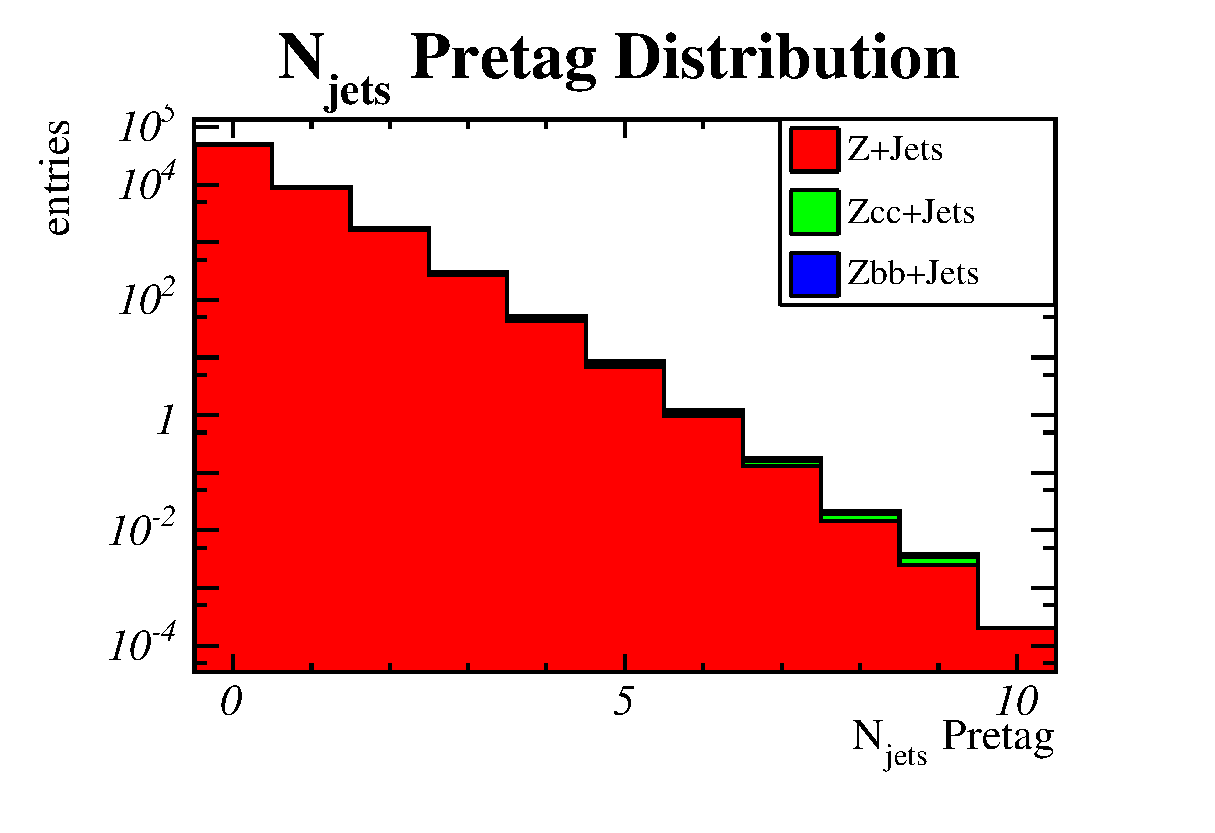
\includegraphics[width=0.6\textwidth]{pics/njet_alpgenonly.eps}
  \end{center}
  \caption{Distribution of the number of jets in events with a
    reconstructed $Z$ from the combination \alp \Zj, SM \ttbar, and
    diboson MC samples.}
  \label{fig:zjets}
\end{figure}

In Fig.~\ref{fig:alpdata}, a comparison of the predictions of the
\alp, SM \ttbar, and dibosons MC samples with data for events with a
$Z$ and three or fewer jets is shown.  The MC simulation
underestimates the number of jets by 15\% already for
$Z+3\:$jets. Therefore we developed a second technique to estimate the
\Zj background that is more data-driven and based on the mass $\chi^2$
described in Section~\ref{section:masschi2}. The separation of signal
from background events as a function of $\chi^2$ is shown in
Fig.~\ref{fig:chi2_separation}. The good separation and the
approximate independence of the background shape of the parton
multiplicity in the \Zj MC leads to the idea of extending the
unblinded area of the analysis to the tail of the $\chi^2$
distribution. For example, a cut of $\sqrt{\chi^2}>3$ would accept
only 3\% of the FCNC signal, but 29\% of the \Zj background. Note that
the $\chi^2$ shape of all background samples is very similar.

As a data-driven method to determine the \Zj background, we fit data
to the high-$chi^2$ tail and extrapolate to the signal region of low
$chi^2$ using the MC shape of the \Zj distribution.  With a cut of
$\sqrt{\chi^2}>3$ we obtain $151 \pm 28$ events, and with a cut of
$\sqrt{\chi^2}>3.2$, the yield is $119 \pm 21$. We take the average of
these two numbers as the background prediction from the mass $\chi^2$,
and the larger of the two uncertainties: $135 \pm 28$ events.


\begin{figure}[t]
  \begin{center}
    \subfigure[]{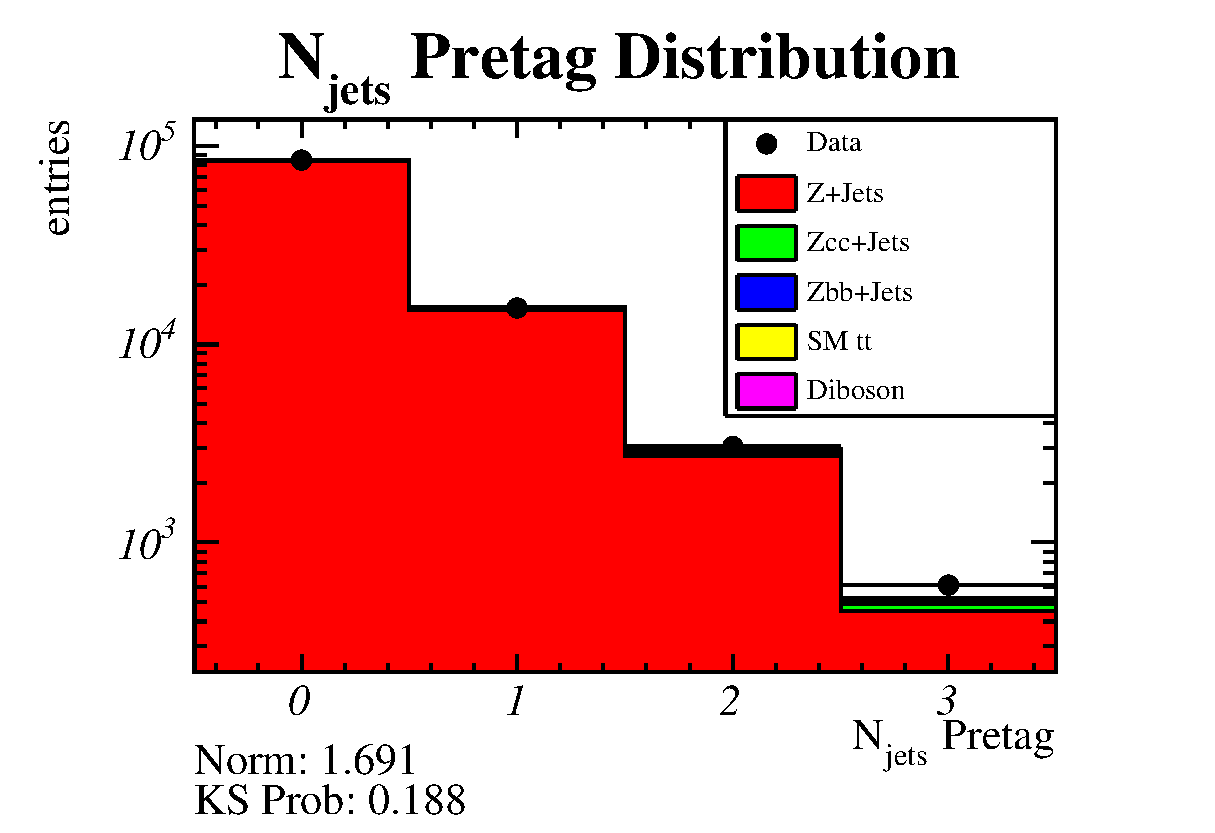
\includegraphics[width=0.48\textwidth]{pics/20070524_njet_nj_pre.eps}}
    \subfigure[]{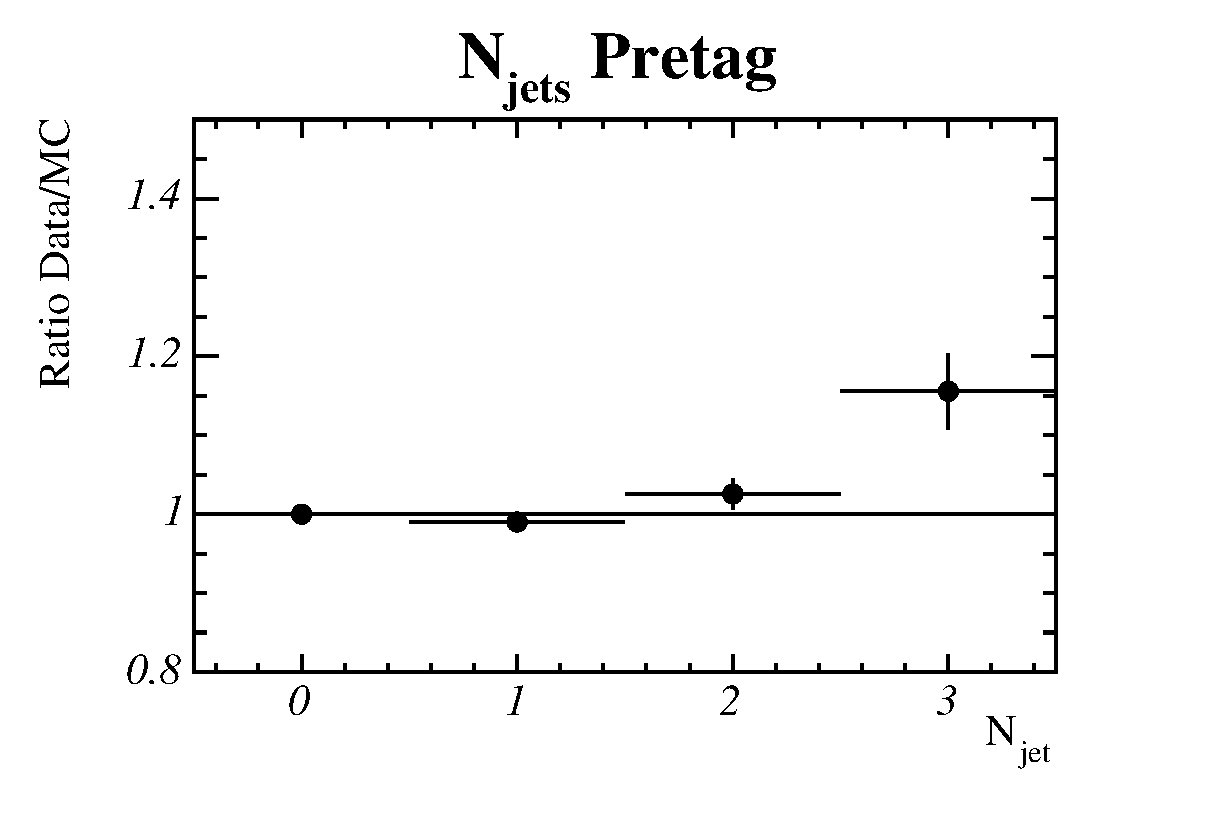
\includegraphics[width=0.48\textwidth]{pics/20070524_njet_ratio_nj_pre.eps}}
  \end{center}
  \caption{Data-MC comparison of the number of jets in events with a
    reconstructed $Z$. (a) Distribution of the number of jets before
    $b$-tagging. (b) ratio of data over MC.}
  \label{fig:alpdata}
\end{figure}

\begin{figure}[t]
  \begin{center}
    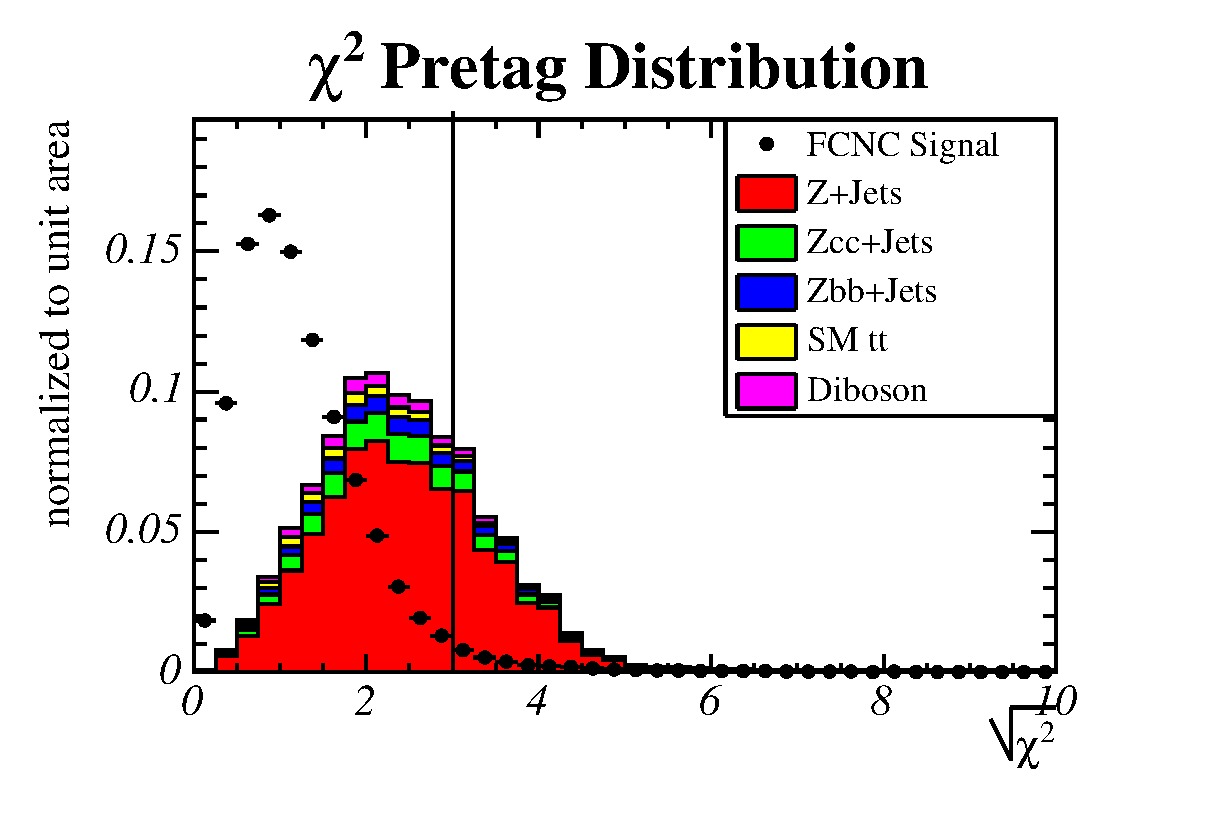
\includegraphics[width=0.6\textwidth]{pics/20070525_chi_pre.eps}
  \end{center}
  \caption{Mass $\chi^2$ distribution of signal and background events. The signal and background samples are normalized to unit area.}
  \label{fig:chi2_separation}
\end{figure}


%In $700\unit{pb^{-1}}$ of
%data, we found 55,775 $Z$ candidates. For $1\unit{fb^{-1}}$, we expect
%80,252 $Z$ candidates. Using the fraction of \Zj in the signal region
%predicted by Monte Carlo, we expect 125 \Zj background events in our
%signal region.


\subsubsection{Heavy Flavor Content and Tagging Rates}
$Z$'s produced in association with heavy flavor ($b$ and $c$) jets
constitute a large portion of the background in the $b$-tagged
sample. We estimate this background by measuring the heavy flavor
fractions, \ie the proportion of \Zj events containing a $b$ or $c$
jet, and the tagging efficiencies for these heavy flavor events. We
measure the contributions to the $b$-tagged background from the MC
samples with $Z+\bbbar+0,1,2$\,partons and $Z+\ccbar+0,1,2$\,partons
and check them in the control region of three or fewer jets in the
data.
%In order to avoid double counting, we discard events
%with heavy flavor in the light flavor samples and events with $b$ jets
%in the $Z$+\ccbar+$n$p samples. The generated \xsects used to weight
%the heavy flavor samples are given in Table~\ref{Znpsigma}. In these
%events, we allow for the possibility of loosing a heavy flavor jet or
%of the two heavy flavor jets merging. 
We divide the sample into events with one heavy flavor jet and events
with two heavy flavor jets. We identify heavy flavor jets by matching
them to $b$ and $c$ hadrons in the OBSP list, as described in
Section~\ref{section:tageff}.  The heavy flavor fractions measured in
the MC simulation are given in Table~\ref{table:Z+HFfrac}.

\begin{table}[t]
\begin{center}
  \caption{\label{table:Z+HFfrac} $Z$ + Heavy Flavor fractions in \alp
    MC. This table gives the fraction of \Zj events (in \%) that
    contain heavy flavor jets, for each physical process, sorted by
    the amount of heavy flavor and number of jets.
    Only statistical errors are given.}
  \vspace{2mm}

  
\small
\begin{tabular}{lD{;}{\pm}{-1}D{;}{\pm}{-1}D{;}{\pm}{-1}D{;}{\pm}{-1}}
\toprule
 {\bf Sample} 
& \multicolumn{1}{c}{\bf 1-jet (\%)}
& \multicolumn{1}{c}{\bf 2-jet (\%)}
& \multicolumn{1}{c}{\bf 3-jet (\%)}
& \multicolumn{1}{c}{\bf 4-jet (\%)} \\
\midrule
$Z\bbbar$, 1 $b$ & 0.8;0.01 & 1.5;0.03 & 2.4;0.05 & 3.3;0.10 \\
$Z\bbbar$, 2 $b$ &  \multicolumn{1}{c}{---} & 1.0;0.02 & 2.1;0.05 & 4.2;0.45 \\
$Z\ccbar$, 1 $c$ & 1.9;0.03 & 3.7;0.07 & 5.5;0.14 & 7.7;0.81 \\
$Z\ccbar$, 2 $c$ &  \multicolumn{1}{c}{---} & 1.4;0.02 & 3.3;0.14 & 5.9;0.17 \\
\bottomrule
\end{tabular}


%   \small\begin{tabular}{lD{;}{\pm}{-1}D{;}{\pm}{-1}D{;}{\pm}{-1}D{;}{\pm}{-1}} \toprule
%     {\bf Sample} & \multicolumn{1}{c}{\bf 1-jet} 
%     & \multicolumn{1}{c}{\bf 2-jet} 
%     & \multicolumn{1}{c}{\bf 3-jet} 
%     & \multicolumn{1}{c}{\bf \boldmath$\geq$\unboldmath 4-jet} \\ 
%     \midrule
%     $Z\bbbar,\, 1\,b$ & 1.5 ; 0.1 & 2.6 ; 0.1 & 3.9 ; 0.2 & 3.8 ; 0.3 \\ 
%     $Z\bbbar,\, 2\,b$ &           & 1.6 ; 0.2 & 3.2 ; 0.3 & 5.6 ; 0.4 \\ 
%     $Z\ccbar,\, 1\,c$ & 0.2 ; 0.0 & 0.5 ; 0.0 & 0.7 ; 0.0 & 1.0 ; 0.1 \\
%     $Z\ccbar,\, 2\,c$ &           & 1.6 ; 0.1 & 3.5 ; 0.1 & 5.7 ; 0.2 \\
%     \bottomrule
%   \end{tabular}
  
\end{center}
\end{table}

We have checked the tagging rates predicted by the \Zj MC simulation
including \Zcc and \Zbb in data.  As the SM \ttbar channels contains
two real $b$ quarks, it contributes significantly to the heavy flavor
content of the background cocktail. To a lesser extend also the
diboson background contributes to the tagging rate. We correct the MC
tagging information by scale factors and mistag probabilities as
described in Section~\ref{section:tageff}. For the comparison we study
the $n$-jet distributions in data and MC simulation.  To keep the
analysis blind, the comparison is restricted to the events with three
or fewer jets.  We keep the contribution from SM \ttbar and diboson
production constant and normalize the \Zj contribution to the pre-tag
data. Fig.~\ref{fig:njet_tag} shows the data-MC comparison. The MC
underestimates the tagging rate in the data by at least 20\%
for all jet bins.

\begin{figure}[t]
  \begin{center}
    \subfigure[]{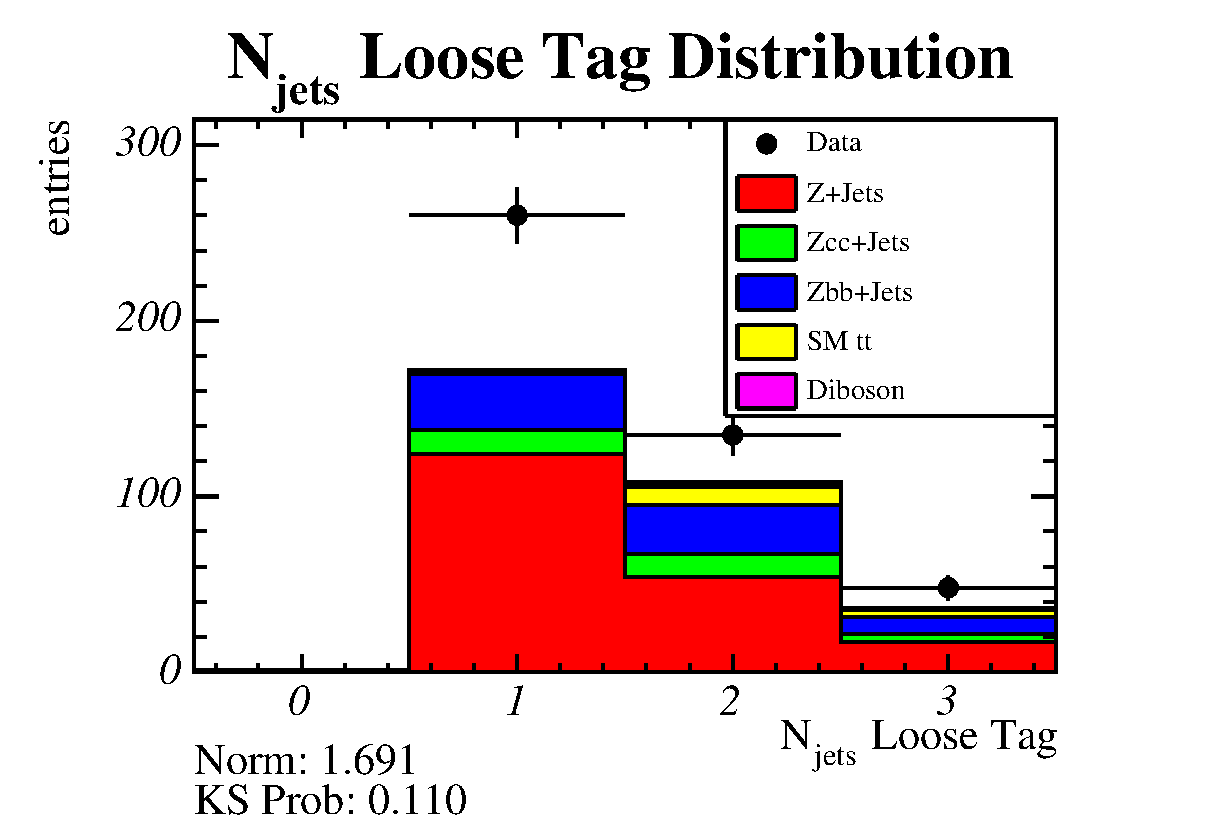
\includegraphics[width=0.48\textwidth]{pics/20070524_njet_nj_loose.eps}}
    \subfigure[]{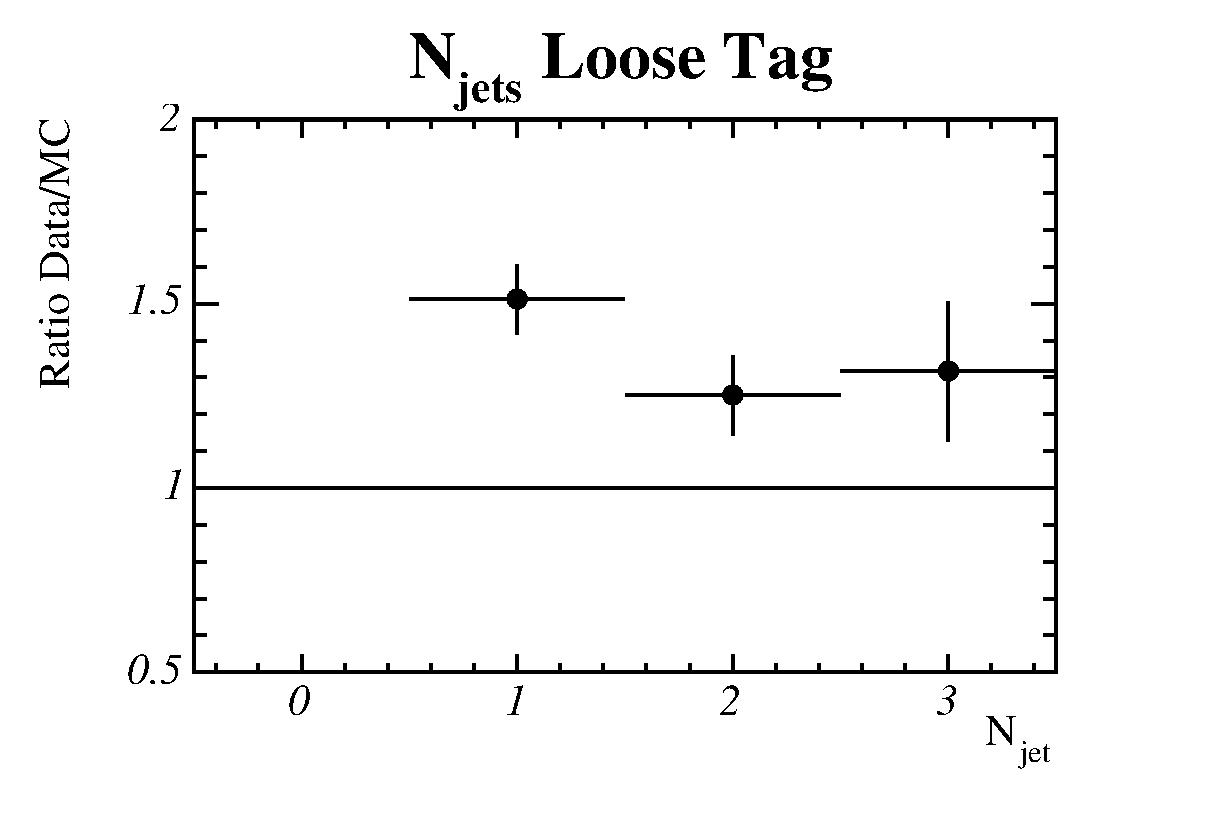
\includegraphics[width=0.48\textwidth]{pics/20070524_njet_ratio_nj_loose.eps}}
  \end{center}
  \caption{Data-MC comparison of the number of tagged events with 1--3
    jets. (a) Distribution of the number of jets for at least one
    loose SECVTX $b$-tag. (b) ratio of data over MC. Note that the MC
    distribution is normalized to the pre-tag data sample.}
  \label{fig:njet_tag}
\end{figure}

The fraction of background events that we expect to be tagged based on
the measurement of heavy flavor fractions in the MC simulation amounts
to 11\%. As we suspect this number to underestimate the real tagging
rate, we double-check it with two different methods. We obtain the
tagging rate from the high-$\chi^2$ sideband by counting the
number of events with a loose SECVTX tag in the region of
$\sqrt{\chi^2}>3$. We count 5 events out of 31, resulting in a tagging
rate of $16\pm7\%$.  As the uncertainty of this data-driven method
is rather large, we check it with a fit to tagging templates.  Tagging
templates are MC templates that contain the MC predictions of the
tagging probabilities separately for the number of jets in the event
and the number of $b$-tags for all background samples and both the
loose and the tight tagger.  Fits to the templates allow subsets of
these degrees of freedom to float. Knowing that the MC does not
predict the jet multiplicities well, we let every jet bin float. The
contribution of SM \ttbar is fixed, the light flavor \Zj sample and
the combination of the \Zcc and the \Zbb samples are allowed to float.
The data together with the fitted template are shown in
Fig.~\ref{fig:tagtemp}. We extract a tagging rate of 14\% from 
this method. We use the average of the results from the $\chi^2$ method
and the template fitting method as our prediction for the 
tagging rate and conservatively estimate the uncertainty such that the
11\% result from the MC heavy flavor fractions is covered:
$15 \pm 4\%$.


\begin{figure}[t]
  \begin{center}
    \subfigure[]{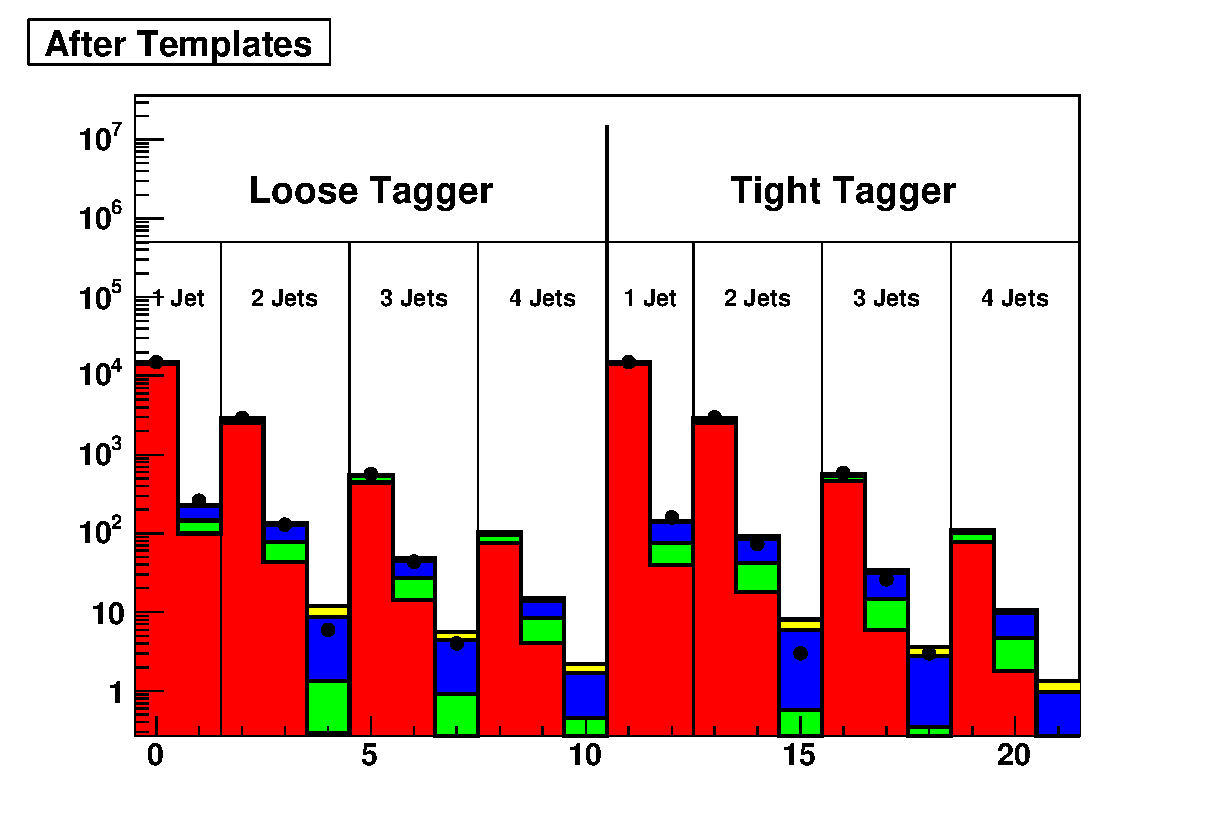
\includegraphics[width=0.48\textwidth]{pics/jettag_Ulrich_hf_after.eps}}
    \subfigure[]{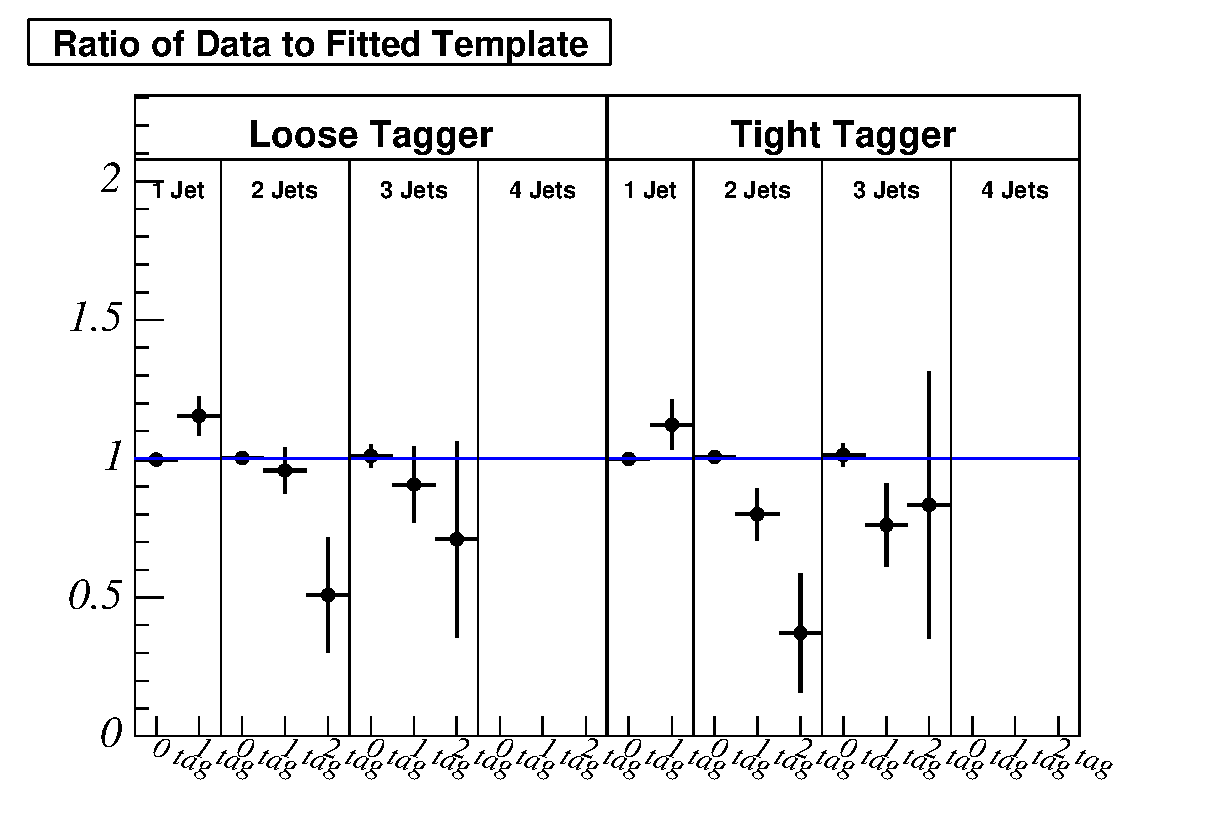
\includegraphics[width=0.48\textwidth]{pics/jettag_Ulrich_hf_ratio.eps}}
  \end{center}
  \caption{Extraction of tagging fractions from a fit to tagging templates. (a) tagging templates fitted to data. (b) Ratio }
  \label{fig:tagtemp}
\end{figure}



%NEEDS UPDATE!!!
%We measure the raw tagging efficiencies for the heavy flavor events in
%the MC simulation for $Z\bbbar$ and $Z\ccbar$ events with one or two
%heavy flavor jets as a function of the jet multiplicity.  The tagging
%efficiencies are then corrected in the same manner as for the signal
%MC, as described in Section~\ref{section:tageff}, \ie taking into
%account $b$-tagging scale factors for identified heavy flavor jets and
%the mistag matrix including $\alpha\beta$ corrections for light flavor
%jets.  The resulting expected tagging efficiencies for heavy flavor
%events in the data are given in Table~\ref{table:HFtagrate}.

%The tagging efficiencies for the heavy flavor events are measured in
%in the MC for each class of events then scaled in a similar manner
%to the tagging efficiency in signal Monte Carlo. The tags in $b$ and
%$c$ jets are scaled down by the loose SECVTX scale factor. In
%addition, light flavor tags are also allowed by adding tags in the
%light flavor jets based on the mistag matrix prediction. This prevents
%the double counting of heavy flavor events with mistags as both heavy
%flavor events and mistag events. 


% \begin{table}[t]
% \begin{center}
%   \caption{\label{table:HFtagrate} Expected $b$-tagging efficiencies
%     in the data (in \%) for $Z$ + Heavy Flavor events, corrected for
%     tagging scale factors and including light flavor tags. Only
%     statistical errors are given.}
%   \vspace{2mm}
  
%   \small\begin{tabular}{lD{;}{\pm}{-1}D{;}{\pm}{-1}D{;}{\pm}{-1}D{;}{\pm}{-1}} \toprule
%     {\bf Sample} & \multicolumn{1}{c}{\bf 1-jet} 
%     & \multicolumn{1}{c}{\bf 2-jet} 
%     & \multicolumn{1}{c}{\bf 3-jet} 
%     & \multicolumn{1}{c}{\bf \boldmath$\geq$\unboldmath 4-jet} \\ 
%     \midrule
%     $Z\bbbar,\, 1\,b$ & 31 ; 2 & 36 ; 3 & 38 ; 4 & 44 ; 6 \\
%     $Z\bbbar,\, 2\,b$ &        & 55 ; 7 & 60 ; 8 & 60 ; 7 \\ 
%     $Z\ccbar,\, 1\,c$ &  9 ; 1 & 11 ; 1 & 14 ; 2 & 15 ; 5 \\
%     $Z\ccbar,\, 2\,c$ &        & 16 ; 1 & 18 ; 1 & 22 ; 1 \\
%     \bottomrule
%   \end{tabular}
% \end{center}
% \end{table}

% In order to obtain the total expected tag rates for \Zj events in the
% data, we multiply the $Z$ + Heavy Flavor fractions and the expected
% tagging efficiencies.  The resulting expected tag rates for \Zj events
% are summarized in Table~\ref{table:Z+Jets_tagrates}.

% \begin{table}
%   \begin{center}
%     \caption{\label{table:Z+Jets_tagrates} The expected tag rates for
%       \Zj events in each $n$-jet bin based on measurements in the MC
%       simulation.}
%     \vspace{2mm}
    
%     \small\begin{tabular}{lD{;}{\pm}{-1}} 
%       \toprule
%       {\bf Sample} & \multicolumn{1}{c}{\bf Expected Tag Rate (\%)} \\ 
%       \midrule
%       $Z+1$\,jet       & 0.5 ; 0.1 \\ 
%       $Z+2$\,jets      & 2.1 ; 0.2 \\
%       $Z+3$\,jets      & 3.9 ; 0.4 \\
%       $Z+\geq 4$\,jets & 6.7 ; 0.5 \\ 
%       \bottomrule
%     \end{tabular}
%   \end{center}
% \end{table}

% In order to verify that the expected tag rate for our signal region
% ($Z+\geq4$\,jet events) is correct, we check the expected tag rates
% for the control region ($Z+1,2,3$\,jet events) against tag rates in
% data. We used the full dataset up to the September 2005 shutdown,
% which is about $695\invpb$ of data. We directly measured the tag rates
% and mistag rates in data. 
% % The measurement of mistag rates in data is described in detail in
% % the next section.
% We also double-check the tag rates and mistag rates for the tight
% tagger against the loose tagger to give us an additional constraint on
% checking the heavy flavor content of the data versus the MC
% simulation. The difference between the tag rate and mistag rate gives
% the rate of tagged heavy flavor events in data. The tag rates, mistag
% rates, and the differences between the two for the loose SECVTX tagger
% are given in Table~\ref{table:loose_datatag} and the tag rates, mistag
% rates and the differences between the two for the tight tagger are
% given in Table~\ref{table:tight_datatag}.  We compared the differences
% in tag rates and mistag rates to the expected tag rate due to heavy
% flavor predicted by Monte Carlo, given in
% Table~\ref{table:Z+Jets_tagrates}. The ratios between data tag rates
% and Monte Carlo predictions are given in
% Table~\ref{table:data_MC_ratios}.

% THE FOLLOWING NEEDS TO BE REVISITED:
% The ratios for the loose and tight
% taggers in events with different number of jets are consistent with
% each other within one sigma and consistently higher than 1.0. The
% average ratio is $1.51 \pm 0.17$. Scaling the predicted tag rate in
% the signal region ($Z\geq 4$\,jet events) by a factor of 1.51 gives a
% rate of $10.12 \pm 1.37\%$. We expect $8.6 \pm 1.12$ tagged events in
% our signal region resulting from $Z$'s produced in association with
% $b$ and $c$ jets.

% \begin{table}[h]
%   \begin{center}
%     \caption{\label{table:loose_datatag} The tag rates, mistag rates, and the differences between the two for the loose SECVTX tagger in \Zj data.}
%     \vspace{2mm}
    
%     \small\begin{tabular}{lD{;}{\pm}{-1}D{;}{\pm}{-1}D{;}{\pm}{-1}} 
%       \toprule
%       {\bf Sample} 
%       & \multicolumn{1}{c}{\bf Tag Rate (\%)}
%       & \multicolumn{1}{c}{\bf Mistag Rate (\%)} 
%       & \multicolumn{1}{c}{\bf Difference (\%)}\\
%       \midrule
%       $Z+1$\,jet & 1.57 ; 0.13 & 0.70 ; 0.11 & 0.87 ; 0.17 \\
%       $Z+2$\,jets & 4.84 ; 0.52 & 1.74 ; 0.26 & 3.10 ; 0.58 \\
%       $Z+3$\,jets & 8.01 ; 1.43 & 3.12 ; 0.47 & 4.89 ; 1.51 \\
%       \bottomrule
%     \end{tabular}
    
%   \end{center}
% \end{table}

% \begin{table}[h]
%   \begin{center}
%     \caption{\label{table:tight_datatag} The tag rates, mistag rates, and the differences between the two for the tight SECVTX tagger in \Zj data.}
%     \vspace{2mm}
    
%     \small\begin{tabular}{lD{;}{\pm}{-1}D{;}{\pm}{-1}D{;}{\pm}{-1}}
%       \toprule
%       {\bf Sample} 
%       & \multicolumn{1}{c}{\bf Tag Rate (\%)}
%       & \multicolumn{1}{c}{\bf Mistag Rate (\%)} 
%       & \multicolumn{1}{c}{\bf Difference (\%)}\\
%       \midrule
%       $Z+1$\,jet & 1.07 ; 0.11 & 0.26 ; 0.04 & 0.81 ; 0.12 \\ 
%       $Z+2$\,jets & 2.76 ; 0.39 & 0.68 ; 0.10 & 2.08 ; 0.40 \\
%       $Z+3$\,jets & 6.35 ; 1.28 & 1.43 ; 0.21 & 4.92 ; 1.30 \\
%       \bottomrule
%     \end{tabular}
%   \end{center}
% \end{table}

% \begin{table}[h]
%   \begin{center}
%     \caption{\label{table:data_MC_ratios} The ratios between tag rates from heavy flavor in data and Monte Carlo for loose and tight SECVTX taggers.}
%     \vspace{2mm}
    
%     \small\begin{tabular}{lD{;}{\pm}{-1}D{;}{\pm}{-1}}
%       \toprule
%       {\bf Sample}
%       & \multicolumn{1}{c}{\bf Ratio (Loose Tagger)}
%       & \multicolumn{1}{c}{\bf Ratio (Tight Tagger)} \\ 
%       \midrule
%       $Z+1$\,jet & 1.67 ; 0.45 & 1.88 ; 0.52 \\ 
%       $Z+2$\,jets & 1.48 ; 0.31 & 1.20 ; 0.27 \\
%       $Z+3$\,jets & 1.27 ; 0.41 & 1.57 ; 0.46 \\
%       \bottomrule
%     \end{tabular}
%   \end{center}
% \end{table}

% \subsubsection[$Z$ + Light Flavor]{\boldmath $Z$\unboldmath{} + Light Flavor}
% Contributions to the tagged background can also result from $Z$'s
% produced in association with light flavor jets, where these jets have
% been mistagged. Although the rate for mistagging light flavor jets is
% small, there are many more events in \Zj events with only light flavor
% jets than events with heavy flavor jets, so a significant portion of
% the tagged background is from $Z$ + Light Flavor events. We estimate
% the mistag probability per event using the mistag matrix and the
% $\alpha\beta$ correction as described in Section~\ref{section:tageff}.
% The average event mistag probabilities for $Z+1,2,3$\,jet events are
% given in Table~\ref{table:loose_datatag} for the loose SECVTX tagger
% and in Table~\ref{table:tight_datatag} for the tight SECVTX tagger.

% THE FOLLOWING NEEDS TO BE REVISITED:
% We extrapolate these mistag rates into our signal region of four or
% more jets (HOW???) and estimate that 6\% of the $Z+\geq 4$\,jet events
% which have only light flavor jets will be tagged (TIGHT TAGGER???). We
% expect 24.3\% of the $Z+\geq 4$\,jet events to contain heavy flavor
% jets (MC estimate + 50\% scaling based on data), i.e. we expect 64 $Z$
% + Light flavor background events in our signal region. Of these, we
% expect 3.9 events to be tagged.
	
%In order to get an estimate for the background from mistagged light
%flavor jets, we ran the {\it negative mistag matrix} on the \Zj sample
%and then apply the rates to the portion of \Zj events which have only
%light flavor jets. The mistag matrix determines the probability for a
%light jet to be tagged by applying the generic jet tag rate to jets in
%the \Zj sample. Details on the mistag matrix are given in CDF Note
%7326~\cite{CDF7326}. This estimate is further corrected by the $\Sigma
%E_{T}$-dependent {\it mistag asymmetry}($\alpha \beta$). These
%corrections account for the imbalance in positive and negative tags
%for light jets and the effect of heavy flavor tags in the generic jet
%samples from which the mistag matrix was derived. More information on
%these corrections can be found in~CDF Note 7585~\cite{CDF7585}.

%Once a mistag probability has been assigned to each jet, we can
%calculate the probability for getting $\geq$1 mistagged jet in each
%event. We do this by subtracting the product of probabilities that
%each jet in the event will not be mistagged from one, i.e.  $1 - \Pi
%(1 - P_{i})$ where $P_i$ is the mistag probability for the
%$i^\mathrm{th}$ jet. 

\subsection[Standard Model \ttbar]{Standard Model \boldmath\ttbar\unboldmath}
Another background contribution to our FCNC search
originates from standard model decays of \ttbar pairs ($\ttbar
\to \Wp b\, \Wm \bbar$). Although there are no real $Z$'s in these
events, the two leptons in dilepton decays can have an invariant mass
reconstructed within our $Z$ mass window. In addition, in lepton+jets
events, a jet can be misidentified as a lepton. These events
contribute if the dilepton mass falls within our $Z$ mass window.

For our studies of the SM \ttbar background, we used 4.7 million
MC-simulated $t\bar{t}$ events generated with the \pyth event
generator at a top quark mass of 175\gevcsq (MC sample:
\texttt{ttop75}). We use the measured \ttbar production \xsect in the
lepton+jets channel using SECVTX $b$-tagged events of $8.8 \pm
1.1\unit{pb}$~\cite{CDF8767} to normalize the MC predictions to
1.12\invfb. The normalized dilepton mass spectrum obtained from the SM
\ttbar MC sample is shown in Fig.~\ref{fig:dilepmass_SMtop}a.  Although
there is no $Z$ mass peak, there are events with a reconstructed
dilepton mass that falls within the $Z$ mass window. The solid line in
Fig.~\ref{fig:dilepmass_SMtop}b shows the distribution of the number of
jets for events inside the $Z$ mass window.  Most of these events have
fewer than four jets. This is because in dilepton events, there are
only two extra hard jets from the decay of the \ttbar pair and in
lepton+jets events, one jet is misidentified as a lepton so there are
only three jets left over. To pass the requirements of four or more
jets, the events need to have extra jets from initial state and final
state radiation. Therefore, the $\geq 4$ jet requirement rejects
91.7\% of this background. Fig.~\ref{fig:dilepmass_SMtop}a shows the 
reconstructed dilepton mass also after requiring $\geq$4 jets. This leaves 
us with $2.4\pm 0.3$ expected events in the signal region in 1.12\invfb, 
rendering SM \ttbar a much smaller background than \Zj ($135\pm 28$ events).


\begin{figure}[t]
  \begin{center}
    \subfigure[]{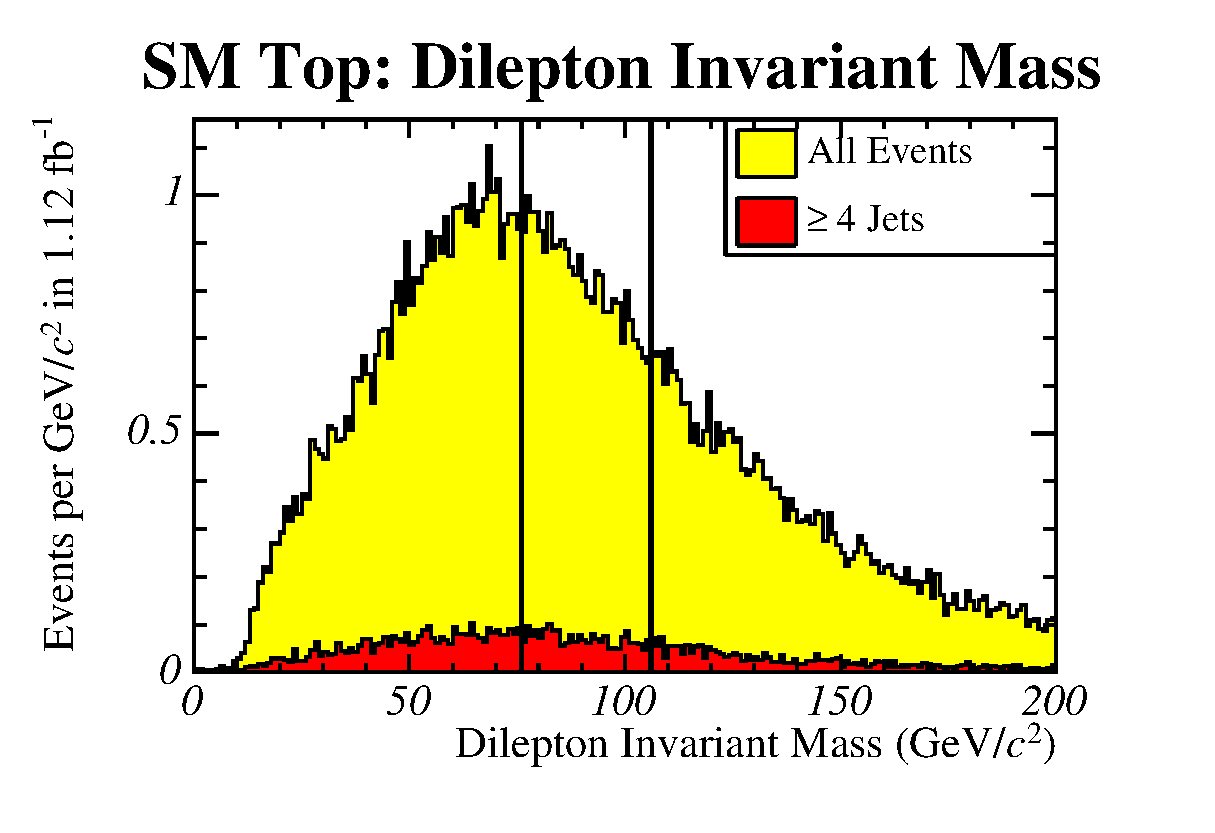
\includegraphics[width=0.48\textwidth]{pics/20070413_smtt_dilepton_mass.eps}}
    \subfigure[]{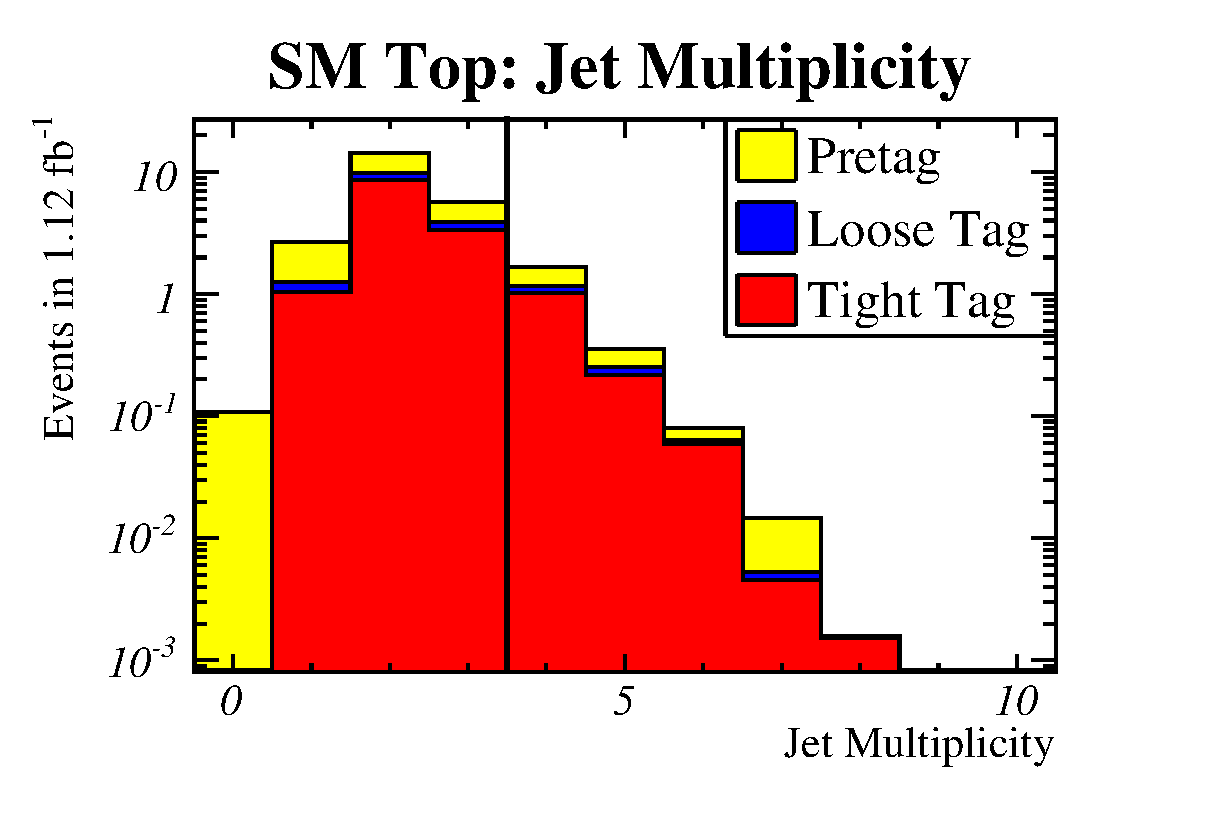
\includegraphics[width=0.48\textwidth]{pics/20070413_smtt_jetmult_tagger.eps}}
  \end{center}
  
  \caption{(a) Reconstructed dilepton mass for all standard model
    \ttbar MC events and events with $\geq 4$~jets. The vertical lines
    show our $Z$ mass selection window. (b) Jet multiplicity for
    standard model \ttbar MC events before $b$-tagging and using the
    loose and tight SECVTX tagger.}
  \label{fig:dilepmass_SMtop}
\end{figure}


Although the contribution of SM \ttbar events to the untagged
background is small, we have to take into account the fact that 
that these events have two $b$-jets in the final state. The efficiency for
finding a $b$-tag is therefore much higher compared to \Zj. As described for the
FCNC signal MC in Section~\ref{section:tageff}, the $b$- and $c$-jet
tags are scaled down by the scale factor, and light flavor tags are
added according to mistag matrix predictions to produce an expected
tagging efficiency in data. In 1.12\invfb of data, we expect $1.6\pm
0.2$ SM \ttbar background events with a loose SECVTX $b$-tag
(compared to an expected number of $20 \pm 6$ tagged \Zj events 
for the loose SECVTX tagger). These results and the MC sample used are
summarized in Table~\ref{table:small_backgrounds}.

\subsection{Dibosons}
We expect background contributions similar to SM \ttbar production
from the production of pairs of gauge bosons (``diboson''), 
$WZ$ and $ZZ$, where events contain real $Z$'s that can
decay into leptons while the other boson is allowed to decay to a pair
of jets, including heavy flavor jets.  Within the detector resolution,
the dijet invariant mass is indistinguishable from the $W$ mass in the
signal MC. There can also be additional jets from initial and final
state radiation which will make these events fall in our signal region
of $Z+4$\,jets.  

We used MC events simulated with \pyth and normalized to the
theoretical \xsects for diboson production to estimate this
background. The theoretical \xsects and their uncertainties are
obtained from the MCFM event generator using MRS98 parton distribution
functions~\cite{Campbell:1999ah}. The samples and \xsects for these
backgrounds are given in Table~\ref{table:small_backgrounds}, along with 
the number of events in 1.12\invfb, before and after tagging. The total
background from both $WZ$ and $ZZ$ diboson production before $b$-tagging 
amounts to $2.9\pm 0.1$ events, larger than the background from SM \ttbar
production. Due to the small fraction of heavy flavor jets, the
diboson background is suppressed in the tagged analysis compared to SM
\ttbar production, with an expected $0.4 \pm 0.0$ events using the
loose SECVTX tagger.

\begin{table}
\small
\begin{center}
\caption{\label{table:small_backgrounds} The dataset names, \xsects, number of events 
  in the MC sample, and expected number of events in 1.12\invfb for both the SM
  \ttbar and the $WZ$ and $ZZ$ diboson samples. Also included in the uncertainty
  calculation is the 6\% luminosity uncertainty.}
\vspace{2mm}

\begin{tabular}{c c D{;}{\pm}{-1} D{;}{,}{-1} D{;}{\pm}{-1} D{;}{\pm}{-1} } 
\toprule
\multicolumn{1}{c}{\bf Sample} & 
\multicolumn{1}{c}{\bf Dataset} & 
\multicolumn{1}{c}{\bf Cross Section} & 
\multicolumn{1}{c}{\bf Generated} &
\multicolumn{1}{c}{\bf Events} &
\multicolumn{1}{c}{\bf Events w/ Loose} \\ 
 & 
\multicolumn{1}{c}{\bf Name} & 
\multicolumn{1}{c}{\bf (pb)} &
\multicolumn{1}{c}{\bf Events} & 
\multicolumn{1}{c}{\bf Pre-Tagged} & 
\multicolumn{1}{c}{\bf SECVTX $b$-Tag} \\

\midrule
SM \ttbar & ttop75 & 8.5;1.1   & 4,719;385 & 2.4;0.3 & 1.6;0.2 \\
$WZ$      & itopwz & 3.96;0.06 & 2,340;145 & 2.0;0.1 & 0.2;<0.1 \\
$ZZ$      & itopzz & 1.58;0.02 & 2,323;812 & 0.8;0.1 & 0.2;<0.1 \\
\bottomrule
\end{tabular}    

  \end{center}
\end{table}

%\begin{table}
%  \begin{center}
%    \caption{\label{table:diboson_bkg} Expected number of background events from %diboson production in 1.12\invfb, before and after $b$-tagging.}
%    \vspace{2mm}%%

%    \small
%    \begin{tabular}{lD{;}{\pm}{-1}D{;}{\pm}{-1}D{;}{\pm}{-1}} \toprule
%      \multicolumn{1}{l}{\bf Sample} & 
%      \multicolumn{1}{c}{\bf Without \boldmath\btag\unboldmath} &
%      \multicolumn{1}{c}{\bf Loose SECVTX \boldmath\btag\unboldmath} &
%      \multicolumn{1}{c}{\bf Tight SECVTX \boldmath\btag\unboldmath} \\
%      \midrule
%      $WW$  & 0.08 ; 0.02 & 0.03 ; 0.01 & 0.03 ; 0.01 \\
%      $WZ$  & 2.15 ; 0.07 & 0.25 ; 0.02 & 0.14 ; 0.02 \\
%      $ZZ$  & 0.89 ; 0.03 & 0.18 ; 0.01 & 0.14 ; 0.01 \\
%      \midrule
%      Total & 3.12 ; 0.08 & 0.45 ; 0.03 & 0.30 ; 0.02\\
%      \bottomrule
%    \end{tabular}
%  \end{center}
%\end{table}

\subsection[$W$ + Jets]{\boldmath $W$\unboldmath{} + Jets}
Another source of background to the FCNC signal comes from the
production of $W$'s in association with jets, \Wj. \Wj events are 
abundant at CDF; the ratio of the \xsects of $W+(n+1)$ jets to 
$Z+n$ jets is approximately 60\%~\cite{TopXSec}. Unlike
the \Zj background, \Wj events require the charged lepton from 
the decay $W\to\ell\nu$ and a jet misidentified as a lepton to 
reconstruct with an invariant mass within the $Z$ mass window. 
Factoring in the probability that this jet becomes
misidentified as lepton decreases this background with respect to
\Zj even further.

We employ different methods to estimate the background from \Wj events
in \ee and \mm final states.  For dimuon events, it is sufficient to
estimate the number of background events from the number of same-sign
muon pairs (or muon-track pairs) that fall into the $Z$ mass window.
We found only 15 same-sign $Z$ candidates in a sample corresponding to
$700\invpb$ of integrated luminosity. None of the events contained
four or more jets; therefore, we conclude that the background from
$W\rightarrow \mu\nu$ + jets events is negligible for our analysis.  
For the electron sample, using same-sign $Z$ candidates is not sufficient 
to estimate the \Wj background. There is a significant contributions to 
the same-sign $Z$ candidates from phoenix electrons whose charge sign was
misidentified. In addition, bremsstrahlung photons radiated from one
or both electrons from the $Z$ decay can be converted into \ee pairs
in the detector material (``trident electrons''), such that three electron 
tracks can be reconstructed per $Z$ leg. One of the electrons has
opposite charge to the original electrons.  We use both the data and
the MC simulation to predict the number of same sign \Zee events we
expect.

The main technique to estimate the \Wj background in \Zee is to study
same-sign electron-muon pairs with an invariant mass falling into the
our $Z$ mass window.  The dominant source of same-sign $e\mu$ pairs is
\Wj decays in which the $W$ decays into $\mu\nu$ and one of the jets
is misidentified as an electron. The charge sign of the muon can be
trusted because the background in \Zmm is negligible. We expect the
same number of same-sign and opposite-sign $e\mu$ pairs from these
decays. To infer the number of same sign \ee pairs from the number of
same-sign $e\mu$ pairs, we have to take into account that the
acceptances for muon identification are different than those for
electron identification. We scale the number of events we find in the
full 1.12\invfb dataset by the ratio $\mathcal{R}$ of the acceptances
$\mathcal{A}$ for $W$ decays into $e\nu$ and $\mu\nu$ final
states~\cite{Acosta:2004uq}:

\begin{equation}
{\mathcal R} = 
\frac{ {\mathcal A}( W \rightarrow e \nu ) }
{{\mathcal A} ( W \rightarrow \mu \nu ) } = 1.217 \pm 0.026.
\end{equation}

The expected number of background events are compared to the number of
opposite-sign \Zee for three and fewer jets in
Table~\ref{table:wjets_bkg}. The fraction of such events is $6\times
10^{-4}$ such that they can be safely neglected.  Note that our method
to estimate the \Wj background does not include track leptons. We
believe that our conclusion that the \Wj background is negligible is
not changed if track leptons are included.

\begin{table}
  \begin{center}
    \caption{\label{table:wjets_bkg} Expected number of events from
      \Wj production in 1.12\invfb in events with three or fewer jets,
      before and after $b$-tagging. The number is estimated from the
      number of same-sign $e\mu$ pairs in the data and compared to the
      number of opposite-sign (OS) \Zee candidates.}
    \vspace{2mm}

    \small
    \begin{tabular}{lD{;}{\pm}{-1}D{;}{\pm}{-1}D{;}{\pm}{-1}D{,}{,}{-1}} \toprule
      \multicolumn{1}{l}{\bf Sample} & 
      \multicolumn{1}{c}{\bf Without \boldmath\btag\unboldmath} &
      \multicolumn{1}{c}{\bf Loose \boldmath\btag\unboldmath} &
      \multicolumn{1}{c}{\bf Tight \boldmath\btag\unboldmath} &
      \multicolumn{1}{c}{\bf OS \boldmath\Zee\unboldmath} \\
      \midrule
      CEM   &  2.4 ; 1.7 & 0.02 ; 0.16 & \multicolumn{1}{c}{not detectable} & 19,325 \\
      PHX   & 21.9 ; 5.2 & 0.04 ; 0.19 & \multicolumn{1}{c}{not detectable} & 22,107 \\
      \midrule
      Total & 24.3 ; 5.5 & 0.06 ; 0.25 & \multicolumn{1}{c}{not detectable} & 41,432 \\
      \bottomrule
    \end{tabular}
  \end{center}
\end{table}

We have double-checked the results of our \Wj background estimate by
two alternative methods that rely more on MC simulations. For both
methods we use an inclusive \Zee MC sample generated with \pyth
(\texttt{zewk6d}) to subtract the number of same-sign $Z$ candidates
expected from charge misidentification and tridents in real \Zee events
from the number of same-sign $Z$ candidates in the data.  In the first
method we obtain the ratio of same-sign to opposite-sign $Z$
candidates from the MC simulation,

\begin{equation}
N_{\mathrm{bkg}}^\mathrm{data} = N_{Z,\mathrm{SS}}^\mathrm{data} - \frac{N_{Z,\mathrm{SS}}^\mathrm{MC}}{N_{Z,\mathrm{OS}}^\mathrm{MC}} \cdot N_{Z,\mathrm{OS}}^\mathrm{data}.
\end{equation}

For the second method we assume that the fraction of tridents in the same-sign $Z$ candidates is correctly modeled in the MC simulation:

\begin{equation}
N_{\mathrm{bkg}}^\mathrm{data} = N_{Z,\mathrm{SS}}^\mathrm{data} - \frac{N_{Z,\mathrm{SS}}^\mathrm{MC}}{N_{\mathrm{trident,OS}}^\mathrm{MC}} \cdot N_{\mathrm{trident,OS}}^\mathrm{data}.
\end{equation}

We find expected background rates of 0.01--0.04 with these methods,
more than an order of magnitude larger than the result obtained with
our main technique. Note however that these methods are conservative
because both the effects of charge misidentification and the amount of
material in the detector giving rise to tridents tend to be
underestimated in the MC. The conclusion that the \Wj background is
negligible remains valid.

\subsection{Background Summary}
In summary, the main background for the search for the FCNC decay \tZq
comes from $Z$ boson production in association with jets. We found
that the background coming from SM \ttbar production and diboson
production is small, and contributions from \Wj events are
negligible. The expected number of background events in our 1.12\invfb
dataset is summarized in Table~\ref{table:bkg_summary}.


\begin{table}
  \begin{center}
    \caption{\label{table:bkg_summary} Summary of all background
      contributions to the search for the FCNC decay \tZq. Given are
      the expected numbers of background events in 1.12\invfb.}
    \vspace{2mm}

    \small
    \begin{tabular}{lD{;}{\pm}{-1}D{;}{\pm}{-1}D{;}{\pm}{-1}} \toprule
      \multicolumn{1}{l}{\bf Source} & 
      \multicolumn{1}{c}{\bf Without \boldmath\btag\unboldmath} &
      \multicolumn{1}{c}{\bf Loose SECVTX\boldmath\btag\unboldmath} \\
      \midrule
      \Zj                   & 135;28      & 20 ; 6  \\ 
      Standard Model \ttbar & 2.4 ; 0.3 & 1.6  ; 0.2 \\
      Diboson               & 2.8 ; 0.1 & 0.4  ; <0.1 \\
      \Wj                   & \multicolumn{1}{c}{$<0.1$} 
      & \multicolumn{1}{c}{negligible}\\
      \bottomrule
    \end{tabular}
  \end{center}
\end{table}


% Systematics
\section{Systematic Uncertainties}
\label{section:systematics}

We have checked a variety of systematic uncertainties both for the
FCNC signal and for the most important source of background events,
the \Zj production. We have also studies the systematics associated 
with the normalization to the lepton+jets \xsect.  The results of our 
studies are summarized in Table~\ref{table:signal_systematics_summary} for the signal
systematics and Table~\ref{table:zjets_systematics_summary} for the
\Zj background systematics.

\subsection{Signal Systematics}

\subsubsection{Luminosity}
As we are normalizing the FCNC acceptance to the acceptance calculated for
the top cross section analysis, the common factor of the luminosity uncertainty
drops out in the ratio.

\subsubsection{Monte Carlo Statistics}
All the MC samples used for this analysis contain a sufficiently large
number of events, so that the uncertainty coming from MC statistics is
reflected by the small statistical uncertainties of the acceptances, and
are therefore negligible.

\subsubsection{\tZq Helicity Reweighing}
\label{section:helicitysystematics}

In order to study the effect of the $Z$ helicity on the FCNC signal
acceptance we have weighted our original MC sample to obtain different
admixtures of longitudinal, left-handed, and right-handed components,
and measured the acceptances for the re-weighted
samples. As generated, the Monte Carlo does not produce a perfectly flat
\costh distribution, as shown in Fig.~\ref{fig:costheta}. Before re-weighting
to the appropriate 65\% longitudinal and 35\% left-handed helicity, we correct
for the approximate flatness by fitting a straight line to the distribution and 
applying a correction factor. Shown  in Fig.~\ref{fig:costheta}b, the original 
distribution is corrected and appropriately re-weighted to the SM expectation. 
Table~\ref{table:reweighting} gives the acceptances for a
collection of re-weighted samples.  Here acceptance is defined as the
ratio of the number of reconstructed signal MC events with a $Z$ candidate 
and four or more jets to the number of generated signal MC
events. Here, we define events with a $Z$ candidates as events with two tight leptons, 
or one tight lepton and one tight track, with scale factors and trigger efficiencies
included, which form a $Z$ in the 76\gevcsq--106\gevcsq mass window. In general, 
the effect of the unknown helicity on the
acceptance is small. The biggest difference occurs between the extreme
cases of a 100\% longitudinal sample and a 100\% left-handed sample,
with a relative acceptance change of 5\%. Since these two values are absolute extremes, 
we consider half the difference, 2.5\%, as the $2\sigma$ systematic uncertainty on the $Z$ helicity.

\begin{table}
  \caption{Change of raw acceptance in the FCNC signal MC for different assumed $Z$ helicities.}
  \label{table:reweighting}
  \begin{center}
    \small
    \begin{tabular}{lD{;}{\pm}{-1}} 
      \toprule
      {\bf Helicity}      & \multicolumn{1}{c}{\bf Acceptance (\%)}  \\ 
      \midrule
      Flat & 17.43;0.05\\
      100\% Longitudinal & 16.93;0.06\\
      100\% Right-Handed & 17.61;0.07\\
      100\% Left-Handed & 17.77;0.07\\
      35\% Left-Handed, 65\% Longitudinal & 17.22;0.06\\
      \bottomrule
    \end{tabular}
  \end{center}
\end{table}

%Another concern for the flat \costh sample is that the \pt shapes of
%the leptons and other distributions will be different than for the
%sample with the correct helicity\footnote{%
%  Strictly speaking, it is the same concern as above, because
%  reweighting the underlying variable \costh corrects the lepton \pt
%%%%%  spectra as well.}.
%We have studied this effect by generating \ttbar events in which one
%top quark decays to a $W$ and a $b$ quark and the other decays to a
%charged Higgs boson $H^+$ and a $b$ quark where the $H^+$ has the same
%mass as $W$ and a vanishing width. Since $t \rightarrow H^+ b$ is not
%a weak decay vertex, \pyth decays the top isotropically instead of
%with a $V\!-\!A$ vertex. We forced the $H^+$ to decay to an electron
%(muon) and a neutrino, and the $W$ to decay to two quarks. We compared
%these events to SM $\ttbar \rightarrow W^+ b\, W^- \bbar$ events in
%which one $W$ decays leptonically and the other decays
%hadronically. Fig.~\ref{fig:higgscheck}a shows the \costh
%distribution of the $t \rightarrow H^+ b$ decay, which is
%flat. Fig.~\ref{fig:higgscheck}b shows the \pt of the lepton from
%the $H^+$ decay compared to the \pt of the lepton from the W decay in
%the SM sample. Fig.~\ref{fig:higgscheck}c shows the \pt of the
%lepton from the $H^+$ decay after the sample has been reweighted to
%have a 70\% longitudinal and 30\% left-handed components compared to
%the \pt of the lepton from the $W$ decay in the Standard Model
%sample. After reweighting the \pt distributions are the same,
%indicating that reweighting the FCNC signal sample will give us the
%correct distributions for \pt of the leptons and other variables.

%\begin{figure}[t]
%\subfigure{}
%\subfigure{}
%\caption{Comparison of kinematic distributions for $t\to H^+ b$ and
%  $t\to W b$: a) \costh for $t\to H^+ b$, b) unweighted lepton \pt, c)
%  weighted lepton \pt.}
%\label{fig:higgscheck}
%\end{figure}

%To estimate the systematic effect of the model-dependent admixture of
%left-handed and right-handed components, we calculate the signal
%acceptance with a fixed longitudinal component of 65\% for left-handed
%to right-handed ratios of 35\%:0\%, 0\%:35\%, and 17.5\%:17.5\%. In
%addition we check the extreme cases of a 100\% left-handed and a 100\%
%right-handed decay. 


\subsubsection{Initial and Final State Radiation}
The modeling of initial state radiation (ISR) and final state
radiation (FSR) in the MC simulation is expected to have an effect on
the number of reconstructed jets. As the signal acceptance requires
four or more reconstructed jets, it is influenced by the amount of ISR
and FSR.  We have generated MC events to study the effect of the
modeling of ISR and FSR on the FCNC signal acceptance. The generated sample
includes 50,000 signal events ( $Z(ll)W(q\overline{q}')$)
each for the scenarios of more ISR, less ISR, more FSR, and less
FSR. The \pyth settings for these samples are those used for similar
studies of the systematics of \ttbar production in Gen5.  The
settings are summarized in Table~\ref{table:isrfsr}. The relevant
\pyth parameters are~\cite{Sjostrand:2003wg}:

\begin{itemize}
\item \texttt{PARP(1)}: nominal value of \LambdaQCD for the running of
\alphas (default: 0.25, units: GeV).
\item \texttt{PARP(61)}: value of \LambdaQCD for the running of
\alphas in space-like shower evolution (default: 0.25, units: GeV).
\item \texttt{PARP(72)}: value of \LambdaQCD for the running of
\alphas in time-like shower evolution (default: 0.25, units: GeV).
\item \texttt{PARP(64)}: $Q^2$ scale times this factor is maximum
parton virtuality in space-like showers (default: 1).
\item \texttt{PARP(71)}: $Q^2$ scale times this factor is maximum
parton virtuality in time-like showers (default: 4).
\end{itemize}


\begin{table}[t]
\small
  \begin{center}
    \caption{\pyth settings for the MC samples to study systematic
      effects due to the amount of initial and final state
      radiation. The \pyth parameters are described in the text.}
    \label{table:isrfsr}
    \vspace{2mm}

  \begin{tabular}{lccccc}
    \toprule
    {\bf Setting} & 
    {\bf PARP(1)}& 
    {\bf PARP(61)}& 
    {\bf PARP(72)}& 
    {\bf PARP(64)} & 
    {\bf PARP(71)} \\
    \midrule
    More ISR & 0.146 & 0.292 & 0.146 & 0.5 & 4.0 \\
    Less ISR & 0.146 & 0.072 & 0.146 & 2.0 & 4.0 \\
    More FSR & 0.146 & 0.146 & 0.292 & 1.0 & 8.0 \\
    Less FSR & 0.146 & 0.146 & 0.076 & 1.0 & 2.0 \\
    \bottomrule
  \end{tabular}
  \end{center}
\end{table}

%NEED ACCEPTANCE NUMBERS, ANY CHANGE IN CHI2 PERFORMANCE?
We have studied the systematic uncertainties due to more or less
ISR/FSR by computing the relative change in acceptance for the
more/less ISR/FSR samples, as compared to 50,000 events from the FCNC
signal MC sample after helicity re-weighting, covering the same run
range. We did not observe a significant change in any kinematic
variable other than the jet multiplicity. The results are summarized
in Table~\ref{table:systematics_isrfsr}. We assign half of the
difference between the largest and the smallest acceptance as the
systematic uncertainty, 0.013.


\begin{table}[t]
  \begin{center}
    \caption{\pyth settings for the MC samples to study systematic
      effects due to the amount of initial and final state
      radiation. The \pyth parameters are described in the text.}
    \label{table:systematics_isrfsr}
    \vspace{2mm}

  \begin{tabular}{lD{;}{\pm}{-1}D{.}{.}{-1}}
    \toprule
    {\bf Setting} & 
%    \multicolumn{1}{c}{\bf Acceptance} &
    \multicolumn{1}{c}{\bf Relative Change} \\
    \midrule
    Default   & 0.0 \\
    \midrule
    More ISR  & +0.001 \\
    Less ISR  & -0.016 \\
    More FSR  & +0.009 \\
    Less FSR  & +0.005 \\
    \bottomrule
  \end{tabular}
  \end{center}
\end{table}

\subsubsection[$B$-Tagging Scale Factor]{\boldmath $B$-Tagging Scale Factor\unboldmath}


%\subsubsection{Parton Distribution Functions}

%\subsubsection{Jet Energy Scale}
%We calculate systematic uncertainties due to the jet energy scale as
%described on the Jet Energy Corrections Web Page~\cite{JES}. We vary
%the parameters of the level-5 jet energy corrections by $\pm 1 \sigma$
%and study the effect on the signal acceptance.

%\subsubsection{Lepton ID}
%We take the systematic uncertainties recommended by the Joint Physics group\dots

\subsection{Background Systematics}

\subsubsection{\alp and MLM Matching}

The \alp MC generator allows to vary several parameters which
influence the MLM matching algorithm and the factorization and
renormalization scale $Q^2$. The central value for the parameters have
been determined partly based on advice by the authors of \alp, partly
by validating \alp against CDF data outside the FCNC signal region. We
have generated test samples for which we varied the \alp settings,
containing 50,000 events each for $Z+0,1,2,3,4$\,partons,
$Z+\ccbar+0,1,2$\,partons, and $Z+\bbbar+0,1,2$\,partons, where the
$Z$ decays into \mm pairs only.


\begin{itemize}
\item{\bf Matching of parton \pt and cluster \et}: \alp is a MC
  generator that handles the production of jets both from hard matrix
  elements and \pyth parton showers. \alp allows to set the
  energy/momentum scale above which jets are generated via matrix
  elements and below which parton showers take over. There are
  separate scales for the parton \pt and the cluster \et, but they are
  commonly taken to be the same, with a default value of
  $(\et,\pt)=(15\gev,15\gevc)$. We have studied samples with
  $(10\gev,10\gevc)$ and $(20\gev,20\gevc)$. Changing the matching cut
  changes the relative \xsects of the $n$-parton subsamples by as much
  as a factor of 20; however, when the samples are combined according
  to their relative cross sections, the effect on the total cross
  section is small, from $-0.012$ for $(10\gev,10\gevc)$ to $+0.015$
  for$(20\gev,20\gevc)$. 
\item {\bf \boldmath $Q^{2}$ \unboldmath scale for parton distribution
    functions}: In \alp, the renormalization and factorization scale
  can be picked.
\item {\bf \boldmath $Q^{2}$ \unboldmath scale for each vertex}: In
  \alp, the value of the QCD coupling $\alphas(Q^2)$ is evaluated at
  every strong vertex individually. There are two options for the
  choice of the energy scale $Q^2=\pt^{~2}$, and $Q^2=m_T^{~2}$, where
  \pt and $m_T$ are the transverse momentum and the transverse mass of
  the vertex. There is an additional parameter to vary the scale of
  $\alphas(Q^2)$ around its central value. We have generated samples
  for both $\pt$ and $m_T$ with scale factors of $0.5$, $1.0$, and
  $2.0$. 
\end{itemize}
To be finalized\dots

%\subsubsection{Heavy Flavor Fractions}


%\subsubsection{Jet Energy Scale}

%\subsubsection{Initial and Final State Radiation}

\subsubsection[$B$-Tagging Scale Factor]{\boldmath $B$-Tagging Scale Factor\unboldmath}
	
%\subsubsection{Lepton ID}

%\subsubsection{Monte Carlo Statistics}

\subsubsection{Luminosity}
Only the diboson background receives its absolute normalization from the integrated luminosity, 
for which we assign a systematic uncertainty of 6\%.

 
\subsection{Systematics Summary}

\begin{table}
  \begin{center}
    \caption{\label{table:signal_systematics_summary} Summary of all systematic
      uncertainties on the signal.}
    \vspace{2mm}

    \small
    \begin{tabular}{cD{;}{\pm}{-1}} 
      \toprule
      \multicolumn{1}{c}{\bf Source} & 
      \multicolumn{1}{c}{\bf Uncertainty} \\
      \midrule
      \\
      \midrule
      Total\\
      \bottomrule
    \end{tabular}
  \end{center}
\end{table}

\begin{table}
  \begin{center}
    \caption{\label{table:zjets_systematics_summary} Summary of all systematic
      uncertainties on the background.}
    \vspace{2mm}

    \small
    \begin{tabular}{cD{;}{\pm}{-1}} 
      \toprule
      \multicolumn{1}{c}{\bf Source} & 
      \multicolumn{1}{c}{\bf Uncertainty} \\
      \midrule
      \\
      \midrule
      Total\\
      \bottomrule
    \end{tabular}
  \end{center}
\end{table}


% Limit Calculations and Optimization
\section{Limits and Optimization}
\label{section:limitsandoptimization}

%%%%%%%%%%%%%%%%%%%%%%% Expected Limits %%%%%%%%%%%%%%%%%%%%%%%%%%%%%
\subsection{Expected Upper Limits}
\label{section:expectedlimits}

When optimizing an analysis, one tries to minimize or maximize a
figure of merit that one believes will lead to the smallest limit or
uncertainty.  Instead of choosing the standard
$\frac{\textrm{signal}}{\sqrt{\textrm{background}}}$, we have decided
to optimize directly on the expected upper limit for two reasons.
First, in order to use
$\frac{\textrm{signal}}{\sqrt{\textrm{background}}}$, one must pick a
value for the signal (we expect none).  One can use the current best
limit or the limit one hopes to achieve, but the choice can strongly
affect the optimization. Second when optimizing using expected upper
limits, the systematic uncertainties are automatically accounted for
correctly.

The idea of expected upper limits is straightforward.  It is the
weighted average of limits where we weight assuming there is no
signal.  The limit calculation itself allows, of course, for signal to
be present.  With a single signal region,

\begin{equation}
  \text{Expected Limit} =\sum\limits_{n_\text{obs}} \underbrace{P(n_\text{obs}|n_\text{back})}_\textrm{weight}\cdot Lim(n_\text{obs}|A,n_\text{back}),
\end{equation}

where $n_\text{obs}$ represents the number of events observed,
$n_\text{back}$ is expected background, $A$ is the signal acceptance
convolved with efficiency, $P(n_\text{obs}|n_\text{back})$ is the
Poisson probability that $n_\text{back}$ background events fluctuated
to $n_\text{obs}$, and $Lim$ is any upper limit calculation.
Generalizing this to $j$ signal regions, we get:

\begin{equation}
  \label {eqn:expectedlimit}
  \text{Expected Limit} =\sum\limits_{\xobs} P(\xobs|\vec{n}_\text{back})\cdot Lim(\xobs|\vec{A},\vec{n}_\text{back}),
\end{equation}

where the vectors in $\vec{n}_\text{obs}$, $\vec{n}_\text{back}$, and
$\vec{A}$ signify the numbers of interest in each of the $j$ signal
regions, {\em e.g.,}

\begin{equation}
  \vec{n}_\text{obs} = \left(
  \begin{array}{c}
    {n_\text{obs}}_1\\
    {n_\text{obs}}_2\\
    \vdots\\
    {n_\text{obs}}_j\\
  \end{array}
  \right)
\end{equation}

In this case the weight is defined as

\begin{equation}
\label{eqn:backest}
P(\xobs|\vec{n}_\text{back}) = \prod^j_{i=1} P({n_\text{obs}}_i| {n_\text{back}}_i)
\end{equation}

if we are not considering systematic uncertainties on the background
estimate.  If we are considering systematic uncertainties, we
calculate this probability by using the generation of random numbers
({\em i.e.,} Gaussian smearing followed by Poisson fluctuations).

%% for $j$ different signal regions.  $\vec{n}_\text{obs}$,
%% $\vec{n}_\text{back}$, and $\vec{A}$ all have the same meaning and the
%% vector signifies that $\vec{n}_\text{obs}$ represents the numbers of
%% observed events in all of the signal regions.



In practice, it is not possible to sum over all possible numbers of
observed events as it includes all positive integers.  The practical
question is how do we know we have summed over enough possibilities?
To solve this problem, we do the following.  

\begin{itemize}

\item Using the background estimate (Equation \ref{eqn:backest}, we
  calculate the distribution of observed events.  Each set of values
  of $n_\text{obs}$ ($\vec{n}_\text{obs}$), and its weight
  ($P(\xobs|\vec{n}_\text{back})$) are called a ``bin.''

\item Sort the bins of $\vec{n}_\text{obs}$ by decreasing probability.

\item Starting with the most probable numbers of events ({\em i.e.,}
  the first bin after sorting), calculate:
 
  \begin{itemize}

    \item the limit, 
    \item the maximum limit yet calculated, $lim_\text{max}$,
    \item the total weight used, \[\text{weight}_\text{sum} = \sum^{n_\text{used}}_{i=1} P(\vec{n}_\text{obs}|\vec{n}_\text{back})\]
    \item the under-estimate of the expected upper limit (Equation
      \ref{eqn:underestimate} below), and
    \item the over-estimate of the estimate of the expected upper limit (Equation
      \ref{eqn:overestimate} below).

  \end{itemize}

\item Continue adding in subsequent bins into the calculations.  Stop
  when the under-estimate and the over-estimate are equal within a
  small number $\delta$ (currently $0.01\%$).

\end{itemize}

For a finite sum, the best value of the expected upper limit is the partial sum divided by the total weight seen:

\begin{equation}
 \text{Expected Limit}_\text{best-estimate} = \frac{\sum\limits^{n_\text{used}}
P(\xobs|\vec{n}_\text{back})\cdot Lim(\xobs|\vec{A},\vec{n}_\text{back})}{ \text{weight}_\text{sum}}
\end{equation}


As the total weight seen goes to 1, this becomes the same formula
shown above in Equation \ref{eqn:expectedlimit}.  The under-estimate
of the expected upper limit is the same as the best estimate without
correcting for the weight we have not yet used:

\begin{equation}
\label{eqn:underestimate}
\text{Expected Limit}_\text{under-estimate} = \sum\limits^{n_\text{used}} P(\xobs|\vec{n}_\text{back})\cdot Lim(\xobs|\vec{A},\vec{n}_\text{back}).
\end{equation}

The over-estimate assumes that the remaining summands will result in
the maximum limit obtained so far.

\begin{eqnarray}
 \text{Expected Limit}_\text{over-estimate} &=& \frac{\sum\limits^{n_\text{used}}
P(\xobs|\vec{n}_\text{back})\cdot Lim(\xobs|\vec{A},\vec{n}_\text{back}) + (1 - \text{weight}_\text{sum}) \cdot lim_\text{max}}{  \text{weight}_\text{sum}} \nonumber\\
\label{eqn:overestimate}
& = & \text{Expected Limit}_\text{best-estimate} + \frac{ (1 - \text{weight}_\text{sum})}{  \text{weight}_\text{sum}} \cdot lim_\text{max}
\end{eqnarray}

An interesting aside: Even if one uses a limit calculation that does
not depend on the choice of metric, there is an inherent metric
dependence in expected limits.  This is not a problem, but implies
that we can not optimize on one variable ({\em e.g.,} $\sqrt{
  {\mathcal B}(t \rightarrow Zc)}$) and then expect an optimal limit
with another ({\em e.g.,} $ {\mathcal B}(t \rightarrow Zc)$).  This is
true whenever two variables that are chosen are not related to each
other with a strictly linear relationship.

%%%%%%%%%%%%%%%%%%%%%%% Scanning Expected Limits %%%%%%%%%%%%%%%%%%%%%%%%%%
\subsection{Scanning Expected Upper Limits}
\label{section:scanexpected}

Optimizing by scanning expected upper limits is very similar to any
other optimization technique.  The main steps are:

\begin{itemize}

  \item Tighten the event selection gradually by moving the cut value
    for the variable in question.

  \item Recalculate all background and acceptance numbers with new
    event selection.

  \item Calculate new expected limit based on new event selection.

\end{itemize}

As with most analyses, we want to optimize using more than one
variable.  To accomplish this, we do sequential optimizations.  For
example, we first scanned the expected upper limits using the \chisq.
We then changed the base cuts to include the optimal value of \chisq
and then optimized using the transverse mass.  We then dropped the
\chisq selection, added the optimal transverse mass cut, and rescanned
\chisq.  This was repeated for all variables we used to optimize the
selection.

Note that there are two contradictory principles that should be
followed here.

\begin{itemize}

  \item As with any fit, the optimization will converge the fastest if
    we start with an optimal event selection.

  \item As with any fit, we want to make sure we find the global
    minimum in expected limits and not a local minimum.  To ensure
    this, we need to optimize several times starting with different
    variables.

\end{itemize}

%%%%%%%%%%%%%%%%%%%%%%% Feldman-Cousins %%%%%%%%%%%%%%%%%%%%%%%%%%%%%
\subsection{Feldman-Cousins Limits}
\label{section:fclimits}

The standard Feldman-Cousins \cite{FeldmanCousins:1998fc} limit
calculation has been very often used by the high energy physics
community because of its properties:

\begin{itemize}

  \item It guarantees a physical answer.

  \item It guarantees coverage.

  \item It decides if the result is a (single-sided) limit, or a
    measurement (two-sided limit).

  \item It has no metric dependence.

\end{itemize}

A complete summary of the Feldman-Cousins method, including the
inclusion of systematic uncertainties can be found in CDF Note 7400
\cite{CDF7400}.  The general idea can be summed up in two stages:

\begin{itemize}

  \item For each true value, $\mu$, a range of expected observed
    events (confidence belt) is generated.  This is done by
    considering both 

    \begin{itemize}
    \item the probability for observing a given number of events given
      the true value  $\mu$, $P(n_\text{obs}|\mu)$, and

    \item the maximum probability to observe this number of events for
      all values of $\mu$, $P(n_\text{obs}|\mu_\text{best})$
    \end{itemize}

    In the discrete case, the ratio of these two values (likelihood
    ratio) is used to order the bins of observed values. The
    confidence belt is described as the bins are added, ordered from
    high to low in likelihood ratio, until the sum of
    $P(n_\text{obs}|\mu)$ reaches the desired confidence level (95\%
    in this case).

  \item The upper limit is found by locating the true value, $\mu$,
    whose lower range almost contains the number of observed events.
    Likewise, a lower limit is found the locating the true value,
    $\mu$, whose upper range almost contains the number of observed
    events.

\end{itemize}

There are two significant changes to the Feldman-Cousins
implementation as compared to the original Feldman-Cousins paper:
discrete case with multiple signal regions and systematic
uncertainties.

Extending the discrete implementation of Feldman-Cousins with $j$
signal regions is straightforward.  In this case, each {\em bin} of
$\vec{n}_\text{obs}$ is now the set of $j$ counts (the same as with
multiple signal regions and expected limits).
$P(\vec{n}_\text{obs}|\mu)$ is the total probability of observing
$n_i$ in each bin given the true value $\mu$:
  \[P(\xobs|\mu) = \prod_\text{signal regions}^j
  P({n_\text{obs}}_i| \mu) \] The value of
  $P(\vec{n}_\text{obs}|\mu_\text{best})$ can no longer be calculated
  using an analytically.  Instead we perform a minimization using {\em
    Minuit}.


When incorporating systematic uncertainties into the Feldman-Cousins
method, we follow the prescription laid out by an earlier work of
Cousins and Highland \cite{CousinsHighland:1992ch} as well as the
published CDF {\em Measurement of $\frac{B(t\rightarrow Wb)}{B(t
    \rightarrow Wq)}$ at the Collider Detector at Fermilab}
\cite{CDF7400,Acosta:2005Branch}.  Simply put, the only
change is that $P(\vec{n}_\text{obs}|\mu)$ is now calculated by
generating pseudo-experiments: Gaussian smearing of the acceptances,
efficiencies, and backgrounds before Poisson fluctuating the numbers
of observed events.

Unfortunately, this implementation of the Feldman-Cousins method is
computationally expensive.  While not a problem for calculating a
single limit, it is very slow for calculation expected upper limits
when two signal regions are used and even worse for scanning expected
upper limits.  For this reason, we have also implemented a objective
Bayesian limit calculation that profiles the systematic uncertainties.

%%%%%%%%%%%%%%%%%%%%%%% Baysian Limits %%%%%%%%%%%%%%%%%%%%%%%%%%%%%
\subsection{Bayesian Limits}
\label{section:baysianlimits}

To calculate the Bayesian limit, we start with the standard Poisson
likelihood:

\begin{eqnarray}
{\mathcal L}  &=& \prod^\textrm{Signal Regions } P({n_\textrm{obs}}_i | {n_\textrm{sig}}_i + {n_\textrm{back}}_i) \cdot \nonumber\\
&& ~~ \prod^\textrm{Systematics} ~ {{\mathcal G} (\textrm{syst}}_k| {\mu_\textrm{syst}}_k, {\sigma_\textrm{syst}}_k)
\end{eqnarray}

where $ P({n_\textrm{obs}}_i | {n_\textrm{sig}}_i +
{n_\textrm{back}}_i)$ is the Poisson probability and $ {\mathcal G}
(\textrm{syst}_k| {\mu_\textrm{syst}}_k, {\sigma_\textrm{syst}}_k)$ is
a Gaussian penalty term to allow for systematic shifts in acceptances,
backgrounds, etc.

First, we profile the likelihood.  This is done by stepping through
the likelihood on a grid of branching fraction values and maximizing
the likelihood at each value while letting the nuisance parameters
float.  To calculate a limit, we multiply the profiled likelihood
function by a prior (1 between the branching fraction values of 0 and
1) and find where we need to set the limits to have 95\% of the area
under posterior probability curve ({\em i.e.,} the likelihood curve
multiplied by the prior) included.


%%%%%%%%%%%%%%%%%%%%%%% Compare FC and Bayes %%%%%%%%%%%%%%%%%%%%%%%%%%%%%
\subsection{Comparison of Feldman-Cousins and Bayesian  Expected Limits}
\label{section:compBayesFC}

As mentioned above in Section \ref{section:scanexpected}, it is too
computationally expensive to scan expected limits using
Feldman-Cousins with two (or more) signal regions.  We therefore use
the Bayesian limit calculation for scanning expected limits.  Luckily,
we have found that these two expected limit calculations track each
other very well.  While they do not have the exact same answers, they
do consistently peak at the same cut values.

Note that even if they did not track perfectly, this solution would
still be completely reasonable.  The worst case outcome is that we did
not pick the absolutely best optimized point in the event selection
space.  Once the cuts have been chosen, it is not relevant how we
chose them.  This is also true for optimizing without systematic
uncertainties.

%%%%%%%%%%%%%%%%%%%%%%% Large Systematic Shifts %%%%%%%%%%%%%%%%%%%%%%%%%%%%%
\subsection{Stability of The Optimization}
\label{section:compBayesFC}

Because some the the systematic uncertainties are large, we performed
final cross checks to verify that we do have the optimal event
selection.  The result of this check can be seen in Figure
I-didn't-make-it-yet.  In this case, the background estimations that
went into the four cases were identical.  We changed the background
distributions to see the effects on the expected limits.

There are two important conclusions.  First, the expected limit does
depend strongly on the actual background estimation.  This is exactly
as expected.  Second, although there is a strong dependence on the
expected limit from the background estimation, the optimization point
is largely unaffected.  This gives us confidence that we have found
the optimal event selection.



%%%%%%%%%%%%%%%%%%%%%%% Optimization Results %%%%%%%%%%%%%%%%%%%%%%%%%%%%%
\subsection{Final Optimization}
\label{section:optvariables}
We optimized using additional cuts on the transverse momenta of the
jets, the transverse mass \mt, and the mass $\chi^2$ on top of the
base selection. After the optimization and relative to the base cuts,
71\% (56\%) of the tagged (anti-tagged) signal remain as as compared
to 16\% (7\%) of the background. The optimized event selection
criteria are given in Table~\ref{table:finalcuts}.  The best expected
limit using the Bayesian method is 7.4\% $\pm$ 2.2\% and from the
Feldman-Cousins method is 7.1\% $\pm$ 3.0\%.

\begin{table}[t]
\begin{center}
\caption{\label{table:finalcuts} The optimized event selection criteria.}
\vspace{2mm}

\small\begin{tabular}{ll} 
  \toprule
  {\bf Kinematic Variable}    & {\bf Optimized Cut}  \\ 
  \midrule
  Z Mass                      & $\in$ [76 GeV, 106 GeV]\\
  Leading Jet \Et             & 40 \gev \\
  Second Jet \Et              & 30 \gev \\
  Third Jet \Et               & 20 \gev \\
  Fourth Jet \Et              & 15 \gev \\
  Transverse Mass, \mt        & $> 200\gev$ \\
  $\sqrt{\chi^2}$             & $< 1.6$ in $b$-tagged sample, \\ 
                              &  $< 1.35$ in the anti-tagged sample \\
\bottomrule
\end{tabular}
\end{center}
\end{table}

	


% Results and Conclusions
\section{Results and Conclusions}



	


\clearemptydoublepage

% Cross-checks
%\input{crosschecks}

% Conclusions
%\input{conclusions}

% Appendicies
\begin{appendix}
\section{Lepton Selection, Scale Factors, and Trigger Efficiencies}
\label{section:LeptonAppendix}

%%%%%%%%%%%%%%%%%%%%%%%%%%%%%%%%%%%%%%%%%%%%%%%%%%%%%%%%%%%%%%%%%%%%%%%
% JP Tight Central Electron Table 
%%%%%%%%%%%%%%%%%%%%%%%%%%%%%%%%%%%%%%%%%%%%%%%%%%%%%%%%%%%%%%%%%%%%%%%
\begin{table}[h]
\begin{center}
\caption{\label{table:TCE} The standard Joint Physics selection criteria 
for tight central electrons~\cite{JPElectron}.}
\vspace{2mm}

\small\begin{tabular}{ll} 
  \toprule
  {\bf Electron Variable}      & {\bf Base Cut}  \\ 
  \midrule
  Fiducial to CES                     & Yes \\
  From photon conversion              & No \\
  \et                                 & $\geq 20\gev$ \\
  Fractional isolation                & $\leq 0.10$ \\
  $E/p$                               & $\leq 2$ (unless $\pt> 50\gevc$) \\
  $E_\mathrm{Had}$ / $E_\mathrm{Em}$  & $\leq 0.055 + 0.00045 E(\mathrm{GeV})$ \\
  Track $z_0$                         & $\leq 60\unit{cm}$  \\
  Track \pt                           & $\geq 10\gevc$ \\
  Track \lshr                         & $\leq 0.2$ \\
  COT axial superlayer hits           & 2 \\
  COT stereo superlayer hits          & 3 \\
  Hits per COT superlayer             & 5 \\
  CES $\Delta z$                      & $(-3\unit{cm};3\unit{cm})$ \\
  CES $\Delta x $ times charge        & $(-3\unit{cm};<1.5\unit{cm})$ \\
  CES strip $\chi^2$                  & $\leq 10$ \\
\bottomrule
\end{tabular}
\end{center}
\end{table}

%%%%%%%%%%%%%%%%%%%%%%%%%%%%%%%%%%%%%%%%%%%%%%%%%%%%%%%%%%%%%%%%%%%%%%%
% JP Tight Phoenix Electron Table 
%%%%%%%%%%%%%%%%%%%%%%%%%%%%%%%%%%%%%%%%%%%%%%%%%%%%%%%%%%%%%%%%%%%%%%%
\begin{table}[h]
\begin{center}
\caption{\label{table:PHX} The standard Joint Physics selection criteria 
for tight phoenix electrons~\cite{JPElectron}.}
\vspace{2mm}

\small\begin{tabular}{ll} 
  \toprule
  {\bf Electron Variable}            & {\bf Base Cut}  \\ 
  \midrule
  Matched to a Phoenix track         & Yes \\
  \et                                & $\geq 20\gev$ \\
  PES two-dimensional $\eta$         & $ 1.2 < |\eta| < 2.8$ \\
  $E_\mathrm{Had}$ / $E_\mathrm{Em}$ & $\leq 0.05$ \\
  PEM $\chi^2$                       & $\leq 10$ \\
  PES $5\times9$ U and V             & $\geq 0.65$ \\
  Fractional isolation               & $\leq 0.10$ \\
  $\Delta R$ between the PES 
  and PEM centroids                  & $\leq 3.0\unit{cm}$ \\
  Silicon hits                       & $\geq 3$ \\
  Track $z_0$                        & $\leq 60\unit{cm}$ \\
  \bottomrule
\end{tabular}
\end{center}
\end{table}

%%%%%%%%%%%%%%%%%%%%%%%%%%%%%%%%%%%%%%%%%%%%%%%%%%%%%%%%%%%%%%%%%%%%%%%
% JP CMUP/CMX Muon Table
%%%%%%%%%%%%%%%%%%%%%%%%%%%%%%%%%%%%%%%%%%%%%%%%%%%%%%%%%%%%%%%%%%%%%%%
\begin{table}[h]
\begin{center}
\caption{\label{table:muons} The standard Joint Physics selection criteria 
for CMUP and CMX muons~\cite{JPMuon}.}
\vspace{2mm}

\small\begin{tabular}{ll} 
  \toprule
  {\bf Muon Variable}                & {\bf Base Cut}  \\ 
  \midrule
  \pt                                  & $\geq 20\gevc$ \\
  \et                                  & $< 2\gev$ \\
  Sliding addition for $E_\mathrm{Em}$  & $0.115\cdot(p-100(\mathrm{GeV}/c))$ for muons with $p > 100\gevc$ \\
  $E_\mathrm{Had}$ & $< 6\gev$ \\
  Sliding addition for $E_\mathrm{Had}$ & $0.028\cdot(p-100(\mathrm{GeV}/c))$ for muons with $p > 100\gevc$ \\
  Fractional isolation                 &  $\leq 0.10$ \\
  COT axial superlayer hits            & 2 \\
  COT stereo superlayer hits           & 3 \\
  Hits per COT superlayer              & 5 \\
  Track $z_0$ & $\leq$ 60 cm  \\
  Impact parameter $d_0$               & $< 0.02\unit{cm}$ (w/ silicon) or $<0.2\unit{cm}$ (w/o silicon) \\
  CMU $|\Delta x|$                       & $< 7\unit{cm}$, for CMUP \\
  CMP $|\Delta x|$                       & $< 5\unit{cm}$, for CMUP \\
  CMX $|\Delta x|$                       & $< 6\unit{cm}$, for CMX \\
  Fiducial x$_\mathrm{CMP}$             & $< 0\unit{cm}$ \\ 
  Fiducial z$_\mathrm{CMP}$             & $< 0\unit{cm}$\\ 
  Fiducial x$_\mathrm{CMU, CMUP, CMX}$  & $< 0\unit{cm}$\\ 
  Fiducial z$_\mathrm{CMU, CMUP, CMX}$  & $< -3\unit{cm}$\\  
  \bottomrule
\end{tabular}
\end{center}
\end{table}

%%%%%%%%%%%%%%%%%%%%%%%%%%%%%%%%%%%%%%%%%%%%%%%%%%%%%%%%%%%%%%%%%%%%%%%
% L+Track Selectrion for Tight Central Tracks
%%%%%%%%%%%%%%%%%%%%%%%%%%%%%%%%%%%%%%%%%%%%%%%%%%%%%%%%%%%%%%%%%%%%%%%
\begin{table}[h]
\begin{center}
\caption{\label{table:tracks} The standard lepton+track top \xsect
measurement selection criteria for tight track leptons. We do not use
the track \chisq cut. For more information, see CDF note 8696~\cite{CDF8696}.}
\vspace{2mm}

\small\begin{tabular}{ll} 
  \toprule
  {\bf Track Variable}      & {\bf Base Cut}  \\ 
  \midrule
  \pt                         & $\geq 20\gevc$ \\
  Track Isolation             & $> 0.9$ \\
  COT axial superlayer hits   & $\geq 24$ \\
  COT stereo superlayer hits  & $\geq 20$ \\
  Silicon hits                & $\geq 3$,  unless $< 3$ expected \\
  Impact parameter  $d_0$     & $< 0.025\unit{cm}$ ($< 3$ silicon hits) \\
  Impact parameter  $d_0$     & $< 0.25\unit{cm}$ ($> 3$ silicon hits) \\
  Track \chisq                & Not used. \\
  \bottomrule
\end{tabular}
\end{center}
\end{table}

%%%%%%%%%%%%%%%%%%%%%%%%%%%%%%%%%%%%%%%%%%%%%%%%%%%%%%%%%%%%%%%%%%%%%%%
% SF and Trigger Efficiency Table
%%%%%%%%%%%%%%%%%%%%%%%%%%%%%%%%%%%%%%%%%%%%%%%%%%%%%%%%%%%%%%%%%%%%%%%
\begin{table}[h]
\begin{center}
  \caption{\label{table:sf} The scale factors and trigger efficiencies used to scale the MC
    simulation estimates for electron~\cite{CDF8629}, \cite{CDF8614},
    muon~\cite{CDF8618}, and track~\cite{CDF8696} reconstruction. Scale factors are
    run-dependent, and are listed below with the corresponding
    datasets. All datasets together represent the full 1.12\invfb
    sample. The uncertainties shown are statistical uncertainties only.}
\vspace{2mm}
%\small\begin{tabular}{l D{;}{\pm}{-1} D{;}{\pm}{-1} D{;}{\pm}{-1}} 
%\toprule
%{\bf Leptons} 
%& \multicolumn{1}{c}{\bf ``0d'': 333 $\mathbf{pb^{-1}}$ } 
%& \multicolumn{1}{c}{\bf ``0h'': 363 $\mathbf{pb^{-1}}$ } 
%& \multicolumn{1}{c}{\bf ``0i'': 424 $\mathbf{pb^{-1}}$ } \\ 
%\midrule
%CEM               & 0.991;0.004 & 0.985;0.004 & 0.974;0.004 \\ 
%Phoenix           & 0.939;0.004 & 0.941;0.004 & 0.922;0.006 \\
%CMUP              & 0.929;0.003 & 0.984;0.001 & 0.983;0.002 \\
%CMX               & 0.945;0.003 & 0.984;0.001 & 0.985;0.002 \\
%Track Leptons     & 0.936;0.002 & 0.982;0.001 & 0.979;0.002 \\
%\bottomrule
%\end{tabular}
\small
\begin{tabular}{l D{;}{\pm}{-1}D{;}{\pm}{-1}D{;}{\pm}{-1}D{;}{\pm}{-1}}
\toprule
 & {\bf 0d} & {\bf 0h} & {\bf 0i\:1} & {\bf 0i\:2} \\
\midrule
{\bf CEM} & & & & \\
Trigger Efficiency       & 0.962;0.007 & 0.976;0.006 & 0.979;0.004 & 0.959;0.007 \\
Electron ID Scale Factor & 0.991;0.005 & 0.985;0.005 & 0.974;0.004 & 0.974;0.004 \\
\midrule
{\bf CMUP} & & & & \\
Trigger Efficiency       & 0.902;0.004 & 0.919;0.004 & 0.918;0.005 & 0.913;0.006 \\ 
Muon ID Scale Factor     & 0.985;0.004 & 0.989;0.004 & 0.975;0.005 & 0.975;0.006 \\
Muon Reconstruction      & 0.951;0.004 & 0.939;0.004 & 0.941;0.004 & 0.955;0.005 \\
\midrule
{\bf CMX Arches} & & & & \\
Trigger Efficiency       & 0.967;0.004 & 0.955;0.004 & 0.954;0.005 & 0.947;0.006 \\
Muon ID Scale Factor     & 1.014;0.004 & 1.000;0.005 & 1.004;0.006 & 1.000;0.008 \\
Muon Reconstruction       & 0.996;0.002 & 0.993;0.002 & 0.989;0.003 & 0.991;0.003 \\
\midrule
{\bf CMX Miniskirt/Keystone} & & & & \\
Trigger Efficiency       & \multicolumn{1}{c}{--} & 0.772;0.014 & 0.744;0.019 & 0.755;0.023 \\
Muon ID Scale Factor     & \multicolumn{1}{c}{--} & 0.979;0.011 & 0.990;0.013 & 1.001;0.015 \\
Muon Reconstruction      & \multicolumn{1}{c}{--} & 0.933;0.009 & 0.939;0.011 & 0.902;0.016 \\
\midrule
{\bf Tracks} & & & & \\
Track ID Scale Factor    & \multicolumn{4}{c}{$0.954\pm0.011$} \\
\bottomrule
\end{tabular}
\end{center}
\end{table}

%\begin{table}[t]
%\begin{center}
%\caption{\label{table:e_eff} The efficiencies for detecting
%electrons at different trigger levels. Shown only are statistical errors. JENNIFER: REFERENCE???}
%\vspace{2mm}
%\small\begin{tabular}{c D{;}{\pm}{-1} D{;}{\pm}{-1} D{;}{\pm}{-1}} 
%\toprule
%& \multicolumn{1}{c}{\bf Level 1 } 
%& \multicolumn{1}{c}{\bf Level 2 } 
%& \multicolumn{1}{c}{\bf Level 3 } \\ 
%\midrule
%Electrons & 0.983;0.003 & 0.999;0.001 & 0.997;0.001 \\ 
%\bottomrule
%\end{tabular}
%\end{center}
%\end{table}

%\begin{table}[t]
%\begin{center}
%  \caption{\label{table:mu_eff} The efficiencies for triggering muons
%    in different parts of the detector. Efficiencies are
%    run-dependent, and are listed below with the corresponding
%    datasets. The data sets together represent the full 1.12\invfb
%    sample. Shown only are statistical errors. JENNIFER: REFERENCE???}
%\vspace{2mm}
%\small\begin{tabular}{c D{;}{\pm}{-1} D{;}{\pm}{-1} D{;}{\pm}{-1}} 
%\toprule
%{\bf Leptons} 
%& \multicolumn{1}{c}{\bf ``0d'': 333 $\mathbf{pb^{-1}}$ } 
%& \multicolumn{1}{c}{\bf ``0h'' and ``0i'': 787 $\mathbf{pb^{-1}}$ } \\ 
%\midrule
%CMUP & 0.902;0.004 & 0.918;0.003 \\ 
%CMX & 0.967;0.004 & 0.953;0.003 \\
%\bottomrule
%\end{tabular}
%\end{center}
%\end{table}

%%%%%%%%%%%%%%%%%%%%%%%%%%%%%%%%%%%%%%%%%%%%%%%%%%%%%%%%%%%%%%%%%%%%%%%
% L+Jets Acceptance Selectrion Criteria
%%%%%%%%%%%%%%%%%%%%%%%%%%%%%%%%%%%%%%%%%%%%%%%%%%%%%%%%%%%%%%%%%%%%%%%
\begin{table}[h]
\begin{center}
\caption{\label{table:LepJets} Listed are the lepton+jets acceptance
selection criteria.}
\vspace{2mm}

\small\begin{tabular}{ll} 
  \toprule
  {\bf Selection Criteria}      & {\bf Base Cut}  \\ 
  \midrule
  Lepton type                  & Tight central leptons: TCE, CMUP, CMX \\
  Number of tight leptons      & $\geq 1 $ \\
  Number of jets               & exactly 3 \\
  Jet \Et, JCL 5               & $\geq 20\gev$ \\
  Missing \Et cut              & $\geq 30\gev$ \\
  $Z$ veto                     & Yes \\
  Dilepton Veto                & Yes \\
  $|z|$ jet vertex             & $\leq 60\unit{cm}$ \\
  $\Delta z$ lepton-jet vertex  & $\leq 5\unit{cm}$ \\
  $H_T$                        & $\geq 200\gev$ \\
  Number of loose SECVTX tags  & $\geq 2$ loose tags \\
  \bottomrule
\end{tabular}
\end{center}
\end{table}


\clearemptydoublepage

\section{\Zj Samples and Cross Sections}
\label{section:ZjetsAppendix}


\begin{table}[h]
\begin{center}
  \caption{\label{table:Znpsigma} The dataset names, \xsects, and number of
    events for the \Zj samples. The first block gives the $Z$ + Light
    Flavor samples and the second and third block give the $Z$ + Heavy
    Flavor samples.}
\vspace{2mm}
\small\begin{tabular}{lcD{.}{.}{-1}D{;}{,}{-1}} 
  \toprule
  \multicolumn{1}{l}{\bf Sample} & 
  \multicolumn{1}{c}{\bf Dataset Name} & 
  \multicolumn{1}{c}{\bf \xsect (pb)} & 
  \multicolumn{1}{c}{\bf Number of Events} \\ 
\midrule
\Zee+0p & \texttt{ztop0p} & 158   &   513;779 \\ 
\Zee+1p & \texttt{ztop1p} & 21.6  &   536;159 \\
\Zee+2p & \texttt{ztop2p} & 3.47  &   536;159 \\
\Zee+3p & \texttt{ztop3p} & 0.550 &   528;491 \\
\Zee+4p & \texttt{ztop4p} & 0.099 &   525;065 \\
\Zmm+0p & \texttt{ztop5p} & 158   &   536;159 \\ 
\Zmm+1p & \texttt{ztop6p} & 21.6  &   536;159 \\
\Zmm+2p & \texttt{ztop7p} & 3.47  &   530;843 \\
\Zmm+3p & \texttt{ztop8p} & 0.550 &   536;159 \\
\Zmm+4p & \texttt{ztop9p} & 0.099 &   536;159 \\
\midrule
\Zee+\bbbar+0p & \texttt{ztopb0} & 0.511 & 532;205 \\
\Zee+\bbbar+1p & \texttt{ztopb1} & 0.134 & 525;955 \\
\Zee+\bbbar+2p & \texttt{ztopb2} & 0.039 & 405;652 \\
\Zmm+\bbbar+0p & \texttt{ztopb5} & 0.511 & 530;793 \\
\Zmm+\bbbar+1p & \texttt{ztopb6} & 0.134 & 525;695\\
\Zmm+\bbbar+2p & \texttt{ztopb7} & 0.039 & 536;159\\ 
\midrule
\Zee+\ccbar+0p & \texttt{ztopc0} & 1.08  & 699;8619 \\
\Zee+\ccbar+1p & \texttt{ztopc1} & 0.331 & 710;734 \\
\Zee+\ccbar+2p & \texttt{ztopc2} & 0.107 & 663;518 \\
\Zmm+\ccbar+0p & \texttt{ztopc5} & 1.08  & 710;734 \\
\Zmm+\ccbar+1p & \texttt{ztopc6} & 0.331 & 710;734 \\
\Zmm+\ccbar+2p & \texttt{ztopc7} & 0.107 & 705;108 \\
\bottomrule
\end{tabular}
\end{center}
\end{table}

\end{appendix}

\clearemptydoublepage

%\bibliographystyle{myamsalpha}
\bibliographystyle{myamsplain}
\bibliography{top_theory,top_exp,top_mc,top_cdf}


\end{document}
